% =====================================================================
%  What changed between the 20 and 27 September drafts.
%  Thin preamble; each section is its own file under sections/.
%  Every number is \rn{KEY} from numbers.tex (make_numbers.py); every
%  figure is drawn by fig_phaseclock.py or fig_abc.py. Build: make.
% =====================================================================
\documentclass[11pt,a4paper]{article}
\usepackage[T1]{fontenc}
\usepackage[utf8]{inputenc}
\usepackage{lmodern}
\usepackage[margin=2.1cm]{geometry}
\usepackage{amsmath,amssymb}
\usepackage{booktabs}
\usepackage{array}
\usepackage{tabularx}
\usepackage{graphicx}
\graphicspath{{fig/}}
\usepackage[font=small,labelfont=bf]{caption}
\usepackage{enumitem}
\usepackage{xcolor}
\usepackage[colorlinks=true,linkcolor=black,citecolor=black,urlcolor=blue]{hyperref}
\definecolor{accent}{RGB}{122,47,47}

%  the paper's \num, renamed so a report key can never shadow a paper key
\makeatletter
\newcommand{\rn}[1]{%
  \ifcsname rep@num@#1\endcsname
    \csname rep@num@#1\endcsname
  \else
    \PackageError{report}{No generated number named '#1'}{Run make_numbers.py.}%
  \fi}
\makeatother
% GENERATED by make_numbers.py. Do not edit.
% 20 Sept = 1b226f5, 27 Sept = 1aa26ca
\expandafter\def\csname rep@num@audit.p10_c2c8_hi\endcsname{22}
\expandafter\def\csname rep@num@audit.p10_c2c8_lo\endcsname{8}
\expandafter\def\csname rep@num@audit.p10_c9_5pct_frm\endcsname{3.068}
\expandafter\def\csname rep@num@audit.p10_c9_5pct_to\endcsname{2.62}
\expandafter\def\csname rep@num@audit.p10_c9_hi\endcsname{15}
\expandafter\def\csname rep@num@audit.p10_c9_lo\endcsname{7}
\expandafter\def\csname rep@num@audit.p10_collapse_c2\endcsname{0/96}
\expandafter\def\csname rep@num@audit.p10_collapse_hi\endcsname{29}
\expandafter\def\csname rep@num@audit.p10_collapse_lo\endcsname{20}
\expandafter\def\csname rep@num@audit.p10_collapse_n\endcsname{96}
\expandafter\def\csname rep@num@audit.p10_frenal\endcsname{5}
\expandafter\def\csname rep@num@audit.p10_ke_exact10\endcsname{0.213}
\expandafter\def\csname rep@num@audit.p10_ke_exact5\endcsname{0.395}
\expandafter\def\csname rep@num@audit.p10_pair_hi\endcsname{0.951}
\expandafter\def\csname rep@num@audit.p10_pair_lo\endcsname{0.630}
\expandafter\def\csname rep@num@audit.p10_r6_below_audit\endcsname{12}
\expandafter\def\csname rep@num@audit.p10_r6_below_paper\endcsname{18}
\expandafter\def\csname rep@num@audit.p10_r6_nom_audit\endcsname{12}
\expandafter\def\csname rep@num@audit.p10_r6_nom_paper\endcsname{13}
\expandafter\def\csname rep@num@audit.p10_repeat_draws\endcsname{12}
\expandafter\def\csname rep@num@audit.p10_repeat_pts\endcsname{10}
\expandafter\def\csname rep@num@audit.p10_repeat_total\endcsname{120}
\expandafter\def\csname rep@num@audit.p10_screen_drop\endcsname{Five}
\expandafter\def\csname rep@num@audit.p10_screen_total\endcsname{ten}
\expandafter\def\csname rep@num@audit.p10_share_cap20\endcsname{37}
\expandafter\def\csname rep@num@audit.p10_share_capv\endcsname{20}
\expandafter\def\csname rep@num@audit.p10_share_nom\endcsname{83}
\expandafter\def\csname rep@num@audit.p10_width_w\endcsname{1.0}
\expandafter\def\csname rep@num@audit.p12_draws\endcsname{118}
\expandafter\def\csname rep@num@audit.p12_imported_ctrl\endcsname{6.9}
\expandafter\def\csname rep@num@audit.p12_imported_pat\endcsname{12.8}
\expandafter\def\csname rep@num@audit.p12_kappa\endcsname{0.1402}
\expandafter\def\csname rep@num@audit.p12_status_cv\endcsname{14.02}
\expandafter\def\csname rep@num@audit.p12_status_label\endcsname{CORROBORATED BUT NOT PRIMARY-VERIFIED}
\expandafter\def\csname rep@num@audit.r58_10pct_frm\endcsname{0.243}
\expandafter\def\csname rep@num@audit.r58_10pct_to\endcsname{0.189}
\expandafter\def\csname rep@num@audit.r58_cells\endcsname{48}
\expandafter\def\csname rep@num@audit.r58_centring_hi\endcsname{60}
\expandafter\def\csname rep@num@audit.r58_centring_lo\endcsname{54}
\expandafter\def\csname rep@num@audit.r58_dom_comb\endcsname{0.299}
\expandafter\def\csname rep@num@audit.r58_dom_width\endcsname{0.300}
\expandafter\def\csname rep@num@audit.r58_rmse_w\endcsname{0.249}
\expandafter\def\csname rep@num@audit.r58_rmse_wo\endcsname{0.249}
\expandafter\def\csname rep@num@audit.r58_verdicts_n\endcsname{three}
\expandafter\def\csname rep@num@audit.r58_verdicts_w\endcsname{0.3}
\expandafter\def\csname rep@num@audit.r58_width_hi\endcsname{1.0}
\expandafter\def\csname rep@num@audit.r58_width_lo\endcsname{0.3}
\expandafter\def\csname rep@num@calc.A\endcsname{32{,}273}
\expandafter\def\csname rep@num@calc.A_over_6\endcsname{5{,}378.8}
\expandafter\def\csname rep@num@calc.B\endcsname{-3{,}177}
\expandafter\def\csname rep@num@calc.B_dis\endcsname{-327}
\expandafter\def\csname rep@num@calc.Bp_load\endcsname{323}
\expandafter\def\csname rep@num@calc.C\endcsname{-5}
\expandafter\def\csname rep@num@calc.D\endcsname{6{,}000}
\expandafter\def\csname rep@num@calc.Km\endcsname{100}
\expandafter\def\csname rep@num@calc.L\endcsname{322.73}
\expandafter\def\csname rep@num@calc.T\endcsname{14}
\expandafter\def\csname rep@num@calc.assay_pct\endcsname{5}
\expandafter\def\csname rep@num@calc.b_admissible\endcsname{-322.7}
\expandafter\def\csname rep@num@calc.bend\endcsname{38}
\expandafter\def\csname rep@num@calc.bias_slope\endcsname{2.549}
\expandafter\def\csname rep@num@calc.delta6\endcsname{2{,}171.5}
\expandafter\def\csname rep@num@calc.delta6_dis\endcsname{5{,}021.5}
\expandafter\def\csname rep@num@calc.diary_b\endcsname{16.1}
\expandafter\def\csname rep@num@calc.diary_factor\endcsname{1.028}
\expandafter\def\csname rep@num@calc.diary_move\endcsname{106}
\expandafter\def\csname rep@num@calc.dis_pct\endcsname{5}
\expandafter\def\csname rep@num@calc.gate\endcsname{0.20}
\expandafter\def\csname rep@num@calc.h1401_span_h\endcsname{12.5}
\expandafter\def\csname rep@num@calc.ke\endcsname{5}
\expandafter\def\csname rep@num@calc.keKm\endcsname{500}
\expandafter\def\csname rep@num@calc.kem6\endcsname{30}
\expandafter\def\csname rep@num@calc.load_pct\endcsname{5}
\expandafter\def\csname rep@num@calc.locus_slope\endcsname{-8.227}
\expandafter\def\csname rep@num@calc.m_hi\endcsname{8.91}
\expandafter\def\csname rep@num@calc.m_hi_dis\endcsname{35.64}
\expandafter\def\csname rep@num@calc.m_lo\endcsname{3.36}
\expandafter\def\csname rep@num@calc.m_lo_dis\endcsname{4.78}
\expandafter\def\csname rep@num@calc.m_ratio_dis\endcsname{5.40}
\expandafter\def\csname rep@num@calc.m_untreated\endcsname{10.0}
\expandafter\def\csname rep@num@calc.m_untreated_dis\endcsname{54.0}
\expandafter\def\csname rep@num@calc.mbar\endcsname{10}
\expandafter\def\csname rep@num@calc.monthly_step\endcsname{30.4}
\expandafter\def\csname rep@num@calc.mwf\endcsname{6}
\expandafter\def\csname rep@num@calc.n_h14\endcsname{53}
\expandafter\def\csname rep@num@calc.n_h1401\endcsname{53}
\expandafter\def\csname rep@num@calc.n_monthly\endcsname{25}
\expandafter\def\csname rep@num@calc.nontwin_dtheta\endcsname{400}
\expandafter\def\csname rep@num@calc.null_amp300\endcsname{3.7}
\expandafter\def\csname rep@num@calc.null_cross\endcsname{1{,}100}
\expandafter\def\csname rep@num@calc.null_km\endcsname{-100}
\expandafter\def\csname rep@num@calc.null_slope\endcsname{-8.227}
\expandafter\def\csname rep@num@calc.null_theta\endcsname{822.7}
\expandafter\def\csname rep@num@calc.peak\endcsname{6{,}400}
\expandafter\def\csname rep@num@calc.relax_b0\endcsname{29.79}
\expandafter\def\csname rep@num@calc.relax_b400\endcsname{59.96}
\expandafter\def\csname rep@num@calc.thalf\endcsname{3.5}
\expandafter\def\csname rep@num@calc.theta\endcsname{3{,}000}
\expandafter\def\csname rep@num@calc.theta_dis\endcsname{150}
\expandafter\def\csname rep@num@calc.trough\endcsname{400}
\expandafter\def\csname rep@num@calc.twin400_km\endcsname{44.65}
\expandafter\def\csname rep@num@calc.twin400_theta\endcsname{3{,}676.7}
\expandafter\def\csname rep@num@calc.twin_b_last\endcsname{400}
\expandafter\def\csname rep@num@calc.twin_bs\endcsname{-200, 0, +200, +400}
\expandafter\def\csname rep@num@calc.unit_b\endcsname{1}
\expandafter\def\csname rep@num@fus.all_10\endcsname{0.153}
\expandafter\def\csname rep@num@fus.all_5\endcsname{0.183}
\expandafter\def\csname rep@num@fus.c2_10\endcsname{0.198}
\expandafter\def\csname rep@num@fus.c2_5\endcsname{0.200}
\expandafter\def\csname rep@num@fus.c2c8_10\endcsname{0.154}
\expandafter\def\csname rep@num@fus.c2c8_5\endcsname{0.184}
\expandafter\def\csname rep@num@fus.c2c9_10\endcsname{0.198}
\expandafter\def\csname rep@num@fus.c2c9_5\endcsname{0.200}
\expandafter\def\csname rep@num@fus.c8_10\endcsname{0.243}
\expandafter\def\csname rep@num@fus.c8_5\endcsname{0.463}
\expandafter\def\csname rep@num@fus.c8c9_10\endcsname{0.237}
\expandafter\def\csname rep@num@fus.c8c9_5\endcsname{0.449}
\expandafter\def\csname rep@num@fus.c9_10\endcsname{1.577}
\expandafter\def\csname rep@num@fus.c9_5\endcsname{3.060}
\expandafter\def\csname rep@num@fus.cap10\endcsname{10}
\expandafter\def\csname rep@num@fus.cap5\endcsname{5}
\expandafter\def\csname rep@num@fus.n_monthly\endcsname{24}
\expandafter\def\csname rep@num@fus.nseeds\endcsname{24}
\expandafter\def\csname rep@num@fus.p2\endcsname{20}
\expandafter\def\csname rep@num@fus.p2_frac\endcsname{0.20}
\expandafter\def\csname rep@num@fus.p8\endcsname{5.4}
\expandafter\def\csname rep@num@fus.p9\endcsname{10}
\expandafter\def\csname rep@num@fus.rec_10\endcsname{1.581}
\expandafter\def\csname rep@num@fus.rec_5\endcsname{3.068}
\expandafter\def\csname rep@num@fus.seed_hi\endcsname{23}
\expandafter\def\csname rep@num@fus.seed_lo\endcsname{0}
\expandafter\def\csname rep@num@gen.bias\endcsname{audit/t4\_bias\_vs\_scatter.py}
\expandafter\def\csname rep@num@gen.boundary\endcsname{src/model\_C/run.py}
\expandafter\def\csname rep@num@gen.cohort\endcsname{audit/t6\_cohort\_with\_kappa.py}
\expandafter\def\csname rep@num@gen.decision\endcsname{audit/d13\_decision\_therapy.py}
\expandafter\def\csname rep@num@gen.design\endcsname{src/design/run.py}
\expandafter\def\csname rep@num@gen.diet\endcsname{audit/t3\_diet\_modulation.py}
\expandafter\def\csname rep@num@gen.drift\endcsname{an}
\expandafter\def\csname rep@num@gen.fibre\endcsname{src/model\_A/run.py}
\expandafter\def\csname rep@num@gen.frontier\endcsname{audit/u23\_wire\_phase11.py}
\expandafter\def\csname rep@num@gen.kesweep\endcsname{audit/t5\_band\_vs\_ke.py}
\expandafter\def\csname rep@num@gen.kmcost\endcsname{audit/n1\_km\_cost.py}
\expandafter\def\csname rep@num@gen.lattice\endcsname{audit/t11\_phase\_lattice.py}
\expandafter\def\csname rep@num@gen.loadcap\endcsname{audit/t8\_load\_by\_capacity.py}
\expandafter\def\csname rep@num@gen.local\endcsname{src/model\_A/run.py}
\expandafter\def\csname rep@num@gen.margin\endcsname{src/model\_C/run.py}
\expandafter\def\csname rep@num@gen.measured\endcsname{audit/t9\_measured\_load.py}
\expandafter\def\csname rep@num@gen.phaseclock\endcsname{audit/g1\_phase\_clock.py}
\expandafter\def\csname rep@num@gen.profile\endcsname{audit/n6\_profile\_vs\_crb.py}
\expandafter\def\csname rep@num@gen.reduction\endcsname{src/model\_C/run.py}
\expandafter\def\csname rep@num@gen.scope\endcsname{audit/n4\_theta\_scope.py}
\expandafter\def\csname rep@num@gen.structure\endcsname{audit/t7\_structure\_transient.py}
\expandafter\def\csname rep@num@gen.therapy\endcsname{audit/t13\_therapy\_forward.py}
\expandafter\def\csname rep@num@gen.tier1\endcsname{audit/t2\_tier1\_margin.py}
\expandafter\def\csname rep@num@gen.transient\endcsname{audit/t1\_transient\_worth.py}
\expandafter\def\csname rep@num@git.abstract_diff_lines\endcsname{0}
\expandafter\def\csname rep@num@git.assay_commit\endcsname{4669c03}
\expandafter\def\csname rep@num@git.assay_date\endcsname{2026-09-13}
\expandafter\def\csname rep@num@git.c3_commit\endcsname{f328ed4}
\expandafter\def\csname rep@num@git.c3_date\endcsname{2026-09-19}
\expandafter\def\csname rep@num@git.del\endcsname{170}
\expandafter\def\csname rep@num@git.fig6_commits\endcsname{4}
\expandafter\def\csname rep@num@git.fig6_first\endcsname{293816b}
\expandafter\def\csname rep@num@git.fig6_first_date\endcsname{2026-09-21}
\expandafter\def\csname rep@num@git.has_R152\endcsname{yes}
\expandafter\def\csname rep@num@git.has_R155\endcsname{yes}
\expandafter\def\csname rep@num@git.has_R158\endcsname{yes}
\expandafter\def\csname rep@num@git.has_R182\endcsname{yes}
\expandafter\def\csname rep@num@git.has_R22\endcsname{yes}
\expandafter\def\csname rep@num@git.ins\endcsname{684}
\expandafter\def\csname rep@num@git.main_boundary\endcsname{2026-09-22}
\expandafter\def\csname rep@num@git.main_carn\endcsname{2026-09-22}
\expandafter\def\csname rep@num@git.main_crisis\endcsname{2026-09-27}
\expandafter\def\csname rep@num@git.main_exposure\endcsname{2026-09-22}
\expandafter\def\csname rep@num@git.main_factor24\endcsname{2026-09-27}
\expandafter\def\csname rep@num@git.main_lap\endcsname{2026-09-22}
\expandafter\def\csname rep@num@git.main_numerics\endcsname{2026-09-22}
\expandafter\def\csname rep@num@git.main_pattern2\endcsname{2026-09-22}
\expandafter\def\csname rep@num@git.main_readings\endcsname{2026-09-22}
\expandafter\def\csname rep@num@git.main_s4\endcsname{2026-09-27}
\expandafter\def\csname rep@num@git.main_separatrix\endcsname{2026-09-22}
\expandafter\def\csname rep@num@git.main_tier1first\endcsname{2026-09-27}
\expandafter\def\csname rep@num@git.main_verified\endcsname{2026-09-22}
\expandafter\def\csname rep@num@git.ncommits\endcsname{195}
\expandafter\def\csname rep@num@git.new\endcsname{1aa26ca}
\expandafter\def\csname rep@num@git.new_as_corrected\endcsname{5}
\expandafter\def\csname rep@num@git.new_date\endcsname{2026-09-27 21:35 UTC}
\expandafter\def\csname rep@num@git.new_keys\endcsname{393}
\expandafter\def\csname rep@num@git.new_main_pp\endcsname{45}
\expandafter\def\csname rep@num@git.new_supplement_pp\endcsname{65}
\expandafter\def\csname rep@num@git.new_withdrawn\endcsname{6}
\expandafter\def\csname rep@num@git.old\endcsname{1b226f5}
\expandafter\def\csname rep@num@git.old_as_corrected\endcsname{1}
\expandafter\def\csname rep@num@git.old_date\endcsname{2026-09-20 20:07 UTC}
\expandafter\def\csname rep@num@git.old_keys\endcsname{211}
\expandafter\def\csname rep@num@git.old_main_pp\endcsname{39}
\expandafter\def\csname rep@num@git.old_supplement_pp\endcsname{61}
\expandafter\def\csname rep@num@git.old_withdrawn\endcsname{0}
\expandafter\def\csname rep@num@git.orig_boundary\endcsname{2026-09-21}
\expandafter\def\csname rep@num@git.orig_carn\endcsname{2026-09-22}
\expandafter\def\csname rep@num@git.orig_crisis\endcsname{2026-09-27}
\expandafter\def\csname rep@num@git.orig_exposure\endcsname{2026-09-21}
\expandafter\def\csname rep@num@git.orig_factor24\endcsname{2026-09-27}
\expandafter\def\csname rep@num@git.orig_lap\endcsname{2026-09-21}
\expandafter\def\csname rep@num@git.orig_numerics\endcsname{2026-09-14}
\expandafter\def\csname rep@num@git.orig_pattern2\endcsname{2026-09-21}
\expandafter\def\csname rep@num@git.orig_readings\endcsname{2026-09-21}
\expandafter\def\csname rep@num@git.orig_s4\endcsname{2026-09-27}
\expandafter\def\csname rep@num@git.orig_separatrix\endcsname{2026-09-22}
\expandafter\def\csname rep@num@git.orig_tier1first\endcsname{2026-09-27}
\expandafter\def\csname rep@num@git.orig_verified\endcsname{2026-09-14}
\expandafter\def\csname rep@num@git.origc_boundary\endcsname{c585d84}
\expandafter\def\csname rep@num@git.origc_carn\endcsname{ea25f4f}
\expandafter\def\csname rep@num@git.origc_crisis\endcsname{0cccbf9}
\expandafter\def\csname rep@num@git.origc_exposure\endcsname{d811ea8}
\expandafter\def\csname rep@num@git.origc_factor24\endcsname{5a9cd22}
\expandafter\def\csname rep@num@git.origc_lap\endcsname{855e377}
\expandafter\def\csname rep@num@git.origc_numerics\endcsname{c6e7a20}
\expandafter\def\csname rep@num@git.origc_pattern2\endcsname{b1aebd7}
\expandafter\def\csname rep@num@git.origc_readings\endcsname{c778d08}
\expandafter\def\csname rep@num@git.origc_s4\endcsname{0cccbf9}
\expandafter\def\csname rep@num@git.origc_separatrix\endcsname{ea25f4f}
\expandafter\def\csname rep@num@git.origc_tier1first\endcsname{0cccbf9}
\expandafter\def\csname rep@num@git.origc_verified\endcsname{c6e7a20}
\expandafter\def\csname rep@num@git.paper_untouched_after_new\endcsname{0}
\expandafter\def\csname rep@num@git.phase10_added\endcsname{2026-09-26}
\expandafter\def\csname rep@num@git.phase10_commit\endcsname{b1be9c4}
\expandafter\def\csname rep@num@git.phase12_added\endcsname{2026-09-27}
\expandafter\def\csname rep@num@git.phase12_commit\endcsname{16224c3}
\expandafter\def\csname rep@num@git.q15_added\endcsname{2026-09-26}
\expandafter\def\csname rep@num@git.q15_commit\endcsname{827a5ad}
\expandafter\def\csname rep@num@git.q5_added\endcsname{2026-09-26}
\expandafter\def\csname rep@num@git.q5_commit\endcsname{45b2c68}
\expandafter\def\csname rep@num@lnew.alt_amp\endcsname{75}
\expandafter\def\csname rep@num@lnew.alt_cut\endcsname{65}
\expandafter\def\csname rep@num@lnew.alt_gain\endcsname{4.8}
\expandafter\def\csname rep@num@lnew.assay_vs_load_assay\endcsname{14.9}
\expandafter\def\csname rep@num@lnew.assay_vs_load_load\endcsname{6.5}
\expandafter\def\csname rep@num@lnew.b_admissible\endcsname{-272.7}
\expandafter\def\csname rep@num@lnew.basin_max\endcsname{49.6}
\expandafter\def\csname rep@num@lnew.bias_row\endcsname{20}
\expandafter\def\csname rep@num@lnew.breath_cv_pub\endcsname{14.0}
\expandafter\def\csname rep@num@lnew.breath_hi\endcsname{50.84}
\expandafter\def\csname rep@num@lnew.breath_lo\endcsname{0.39}
\expandafter\def\csname rep@num@lnew.breath_mean\endcsname{14.02}
\expandafter\def\csname rep@num@lnew.breath_n\endcsname{fifteen}
\expandafter\def\csname rep@num@lnew.breath_sd\endcsname{12.86}
\expandafter\def\csname rep@num@lnew.c3_corrected\endcsname{As corrected.}
\expandafter\def\csname rep@num@lnew.carn_old_claim\endcsname{the carnitine state is fast relative to the metabolite}
\expandafter\def\csname rep@num@lnew.crisis039_count\endcsname{0}
\expandafter\def\csname rep@num@lnew.crisis_km_lo\endcsname{thirty}
\expandafter\def\csname rep@num@lnew.d2672_sd\endcsname{2.96}
\expandafter\def\csname rep@num@lnew.dec_rho1_err\endcsname{19.1}
\expandafter\def\csname rep@num@lnew.dec_rho1_med\endcsname{0.88}
\expandafter\def\csname rep@num@lnew.diet_gate\endcsname{10}
\expandafter\def\csname rep@num@lnew.dmax_5pct\endcsname{2672}
\expandafter\def\csname rep@num@lnew.dosesens_n\endcsname{10}
\expandafter\def\csname rep@num@lnew.dsweep_dis_best\endcsname{2.75}
\expandafter\def\csname rep@num@lnew.dsweep_dis_booked\endcsname{3.07}
\expandafter\def\csname rep@num@lnew.dsweep_dis_d\endcsname{100}
\expandafter\def\csname rep@num@lnew.dsweep_nom_best\endcsname{0.165}
\expandafter\def\csname rep@num@lnew.dsweep_range_hi\endcsname{30000}
\expandafter\def\csname rep@num@lnew.dsweep_range_lo\endcsname{10}
\expandafter\def\csname rep@num@lnew.dsweep_within\endcsname{three}
\expandafter\def\csname rep@num@lnew.enzyme_x_normal\endcsname{2.18}
\expandafter\def\csname rep@num@lnew.excluded_three\endcsname{three times}
\expandafter\def\csname rep@num@lnew.factor24_count\endcsname{0}
\expandafter\def\csname rep@num@lnew.factor24_old\endcsname{24}
\expandafter\def\csname rep@num@lnew.h28_cut\endcsname{87}
\expandafter\def\csname rep@num@lnew.h28_gain\endcsname{6.5}
\expandafter\def\csname rep@num@lnew.h28_word\endcsname{twenty-eight}
\expandafter\def\csname rep@num@lnew.h7_cost\endcsname{29}
\expandafter\def\csname rep@num@lnew.h7_word\endcsname{seven}
\expandafter\def\csname rep@num@lnew.ke_exact_left\endcsname{0.388}
\expandafter\def\csname rep@num@lnew.ke_gain_dis\endcsname{6.9}
\expandafter\def\csname rep@num@lnew.ke_gain_nom\endcsname{2.1}
\expandafter\def\csname rep@num@lnew.ke_tight\endcsname{5}
\expandafter\def\csname rep@num@lnew.lapfrac_a\endcsname{4}
\expandafter\def\csname rep@num@lnew.lapfrac_b\endcsname{10}
\expandafter\def\csname rep@num@lnew.lapfrac_c\endcsname{25}
\expandafter\def\csname rep@num@lnew.lapfrac_d\endcsname{50}
\expandafter\def\csname rep@num@lnew.lapfrac_e\endcsname{75}
\expandafter\def\csname rep@num@lnew.margin_hi\endcsname{9}
\expandafter\def\csname rep@num@lnew.margin_lo\endcsname{-4}
\expandafter\def\csname rep@num@lnew.misspec_high_hi\endcsname{2.0}
\expandafter\def\csname rep@num@lnew.misspec_high_lo\endcsname{1.3}
\expandafter\def\csname rep@num@lnew.mtol_a\endcsname{15}
\expandafter\def\csname rep@num@lnew.mtol_b\endcsname{40}
\expandafter\def\csname rep@num@lnew.mtol_c\endcsname{160}
\expandafter\def\csname rep@num@lnew.mtolwin_in_abstract\endcsname{0}
\expandafter\def\csname rep@num@lnew.mtolwin_in_question\endcsname{3}
\expandafter\def\csname rep@num@lnew.n20_n\endcsname{20}
\expandafter\def\csname rep@num@lnew.null_amp\endcsname{3.7}
\expandafter\def\csname rep@num@lnew.null_cross\endcsname{1100}
\expandafter\def\csname rep@num@lnew.p_2mc\endcsname{0.84}
\expandafter\def\csname rep@num@lnew.p_c3\endcsname{0.017}
\expandafter\def\csname rep@num@lnew.pairs_181\endcsname{181}
\expandafter\def\csname rep@num@lnew.r22\endcsname{R22}
\expandafter\def\csname rep@num@lnew.reduction_gap_hi\endcsname{25.4}
\expandafter\def\csname rep@num@lnew.reduction_gap_lo\endcsname{3.4}
\expandafter\def\csname rep@num@lnew.relax_b0\endcsname{29.79}
\expandafter\def\csname rep@num@lnew.relax_b400\endcsname{59.96}
\expandafter\def\csname rep@num@lnew.remark4_title\endcsname{The sampling schedule must complete one lap of the dose cycle.}
\expandafter\def\csname rep@num@lnew.route6_below\endcsname{eighteen}
\expandafter\def\csname rep@num@lnew.rr_2mc\endcsname{1.0}
\expandafter\def\csname rep@num@lnew.rr_3hp\endcsname{0.7}
\expandafter\def\csname rep@num@lnew.rr_3hp_ci_hi\endcsname{0.9}
\expandafter\def\csname rep@num@lnew.rr_3hp_ci_lo\endcsname{0.6}
\expandafter\def\csname rep@num@lnew.rr_c3\endcsname{0.6}
\expandafter\def\csname rep@num@lnew.rr_per\endcsname{50}
\expandafter\def\csname rep@num@lnew.s4_title\endcsname{Admissibility, with the evidence for each verdict}
\expandafter\def\csname rep@num@lnew.saudi_founder\endcsname{70.2}
\expandafter\def\csname rep@num@lnew.saudi_pcca\endcsname{81}
\expandafter\def\csname rep@num@lnew.saudi_pcca_n\endcsname{68 of 84}
\expandafter\def\csname rep@num@lnew.scope_5pct_ratio\endcsname{5.40}
\expandafter\def\csname rep@num@lnew.seeds_n\endcsname{twelve}
\expandafter\def\csname rep@num@lnew.seeds_reps\endcsname{four hundred}
\expandafter\def\csname rep@num@lnew.sep_depleted_a\endcsname{1.9}
\expandafter\def\csname rep@num@lnew.sep_depleted_b\endcsname{4.8}
\expandafter\def\csname rep@num@lnew.sep_depleted_c\endcsname{7.3}
\expandafter\def\csname rep@num@lnew.sep_depleted_fill\endcsname{0.8}
\expandafter\def\csname rep@num@lnew.sep_parent_basin_hi\endcsname{18}
\expandafter\def\csname rep@num@lnew.sep_parent_basin_lo\endcsname{10}
\expandafter\def\csname rep@num@lnew.six_routes\endcsname{Six}
\expandafter\def\csname rep@num@lnew.step_off_v\endcsname{14.5}
\expandafter\def\csname rep@num@lnew.t_struct1h\endcsname{one hour}
\expandafter\def\csname rep@num@lnew.t_struct_t15\endcsname{fifteen}
\expandafter\def\csname rep@num@lnew.t_struct_t3\endcsname{three}
\expandafter\def\csname rep@num@lnew.tauc_ratio_hi\endcsname{55}
\expandafter\def\csname rep@num@lnew.tauc_ratio_lo\endcsname{0.52}
\expandafter\def\csname rep@num@lnew.theta_parent\endcsname{300}
\expandafter\def\csname rep@num@lnew.title\endcsname{Design Rules and Limits of Recoverability for}
\expandafter\def\csname rep@num@lnew.turnover_n\endcsname{thirteen}
\expandafter\def\csname rep@num@lnew.turnover_vs\endcsname{twenty-five}
\expandafter\def\csname rep@num@lnew.verified_old_claim\endcsname{the reduction is verified rather than asserted}
\expandafter\def\csname rep@num@lold.alt_amp\endcsname{75}
\expandafter\def\csname rep@num@lold.alt_cut\endcsname{65}
\expandafter\def\csname rep@num@lold.alt_gain\endcsname{4.8}
\expandafter\def\csname rep@num@lold.assay_vs_load_assay\endcsname{14.9}
\expandafter\def\csname rep@num@lold.assay_vs_load_load\endcsname{6.5}
\expandafter\def\csname rep@num@lold.b_admissible\endcsname{-272.7}
\expandafter\def\csname rep@num@lold.bias_both20\endcsname{0.288}
\expandafter\def\csname rep@num@lold.bias_row\endcsname{20}
\expandafter\def\csname rep@num@lold.bias_theta_factor\endcsname{1.028}
\expandafter\def\csname rep@num@lold.breath_cv_pub\endcsname{14.0}
\expandafter\def\csname rep@num@lold.breath_hi\endcsname{50.84}
\expandafter\def\csname rep@num@lold.breath_lo\endcsname{0.39}
\expandafter\def\csname rep@num@lold.breath_mean\endcsname{14.02}
\expandafter\def\csname rep@num@lold.breath_n\endcsname{fifteen}
\expandafter\def\csname rep@num@lold.breath_sd\endcsname{12.86}
\expandafter\def\csname rep@num@lold.c3_corrected\endcsname{As corrected.}
\expandafter\def\csname rep@num@lold.crisis039_count\endcsname{1}
\expandafter\def\csname rep@num@lold.crisis_threshold\endcsname{-0.39}
\expandafter\def\csname rep@num@lold.d2672_sd\endcsname{2.96}
\expandafter\def\csname rep@num@lold.dec_rho1_err\endcsname{17.5}
\expandafter\def\csname rep@num@lold.dec_rho1_med\endcsname{1.03}
\expandafter\def\csname rep@num@lold.diet_gain15_pct\endcsname{7}
\expandafter\def\csname rep@num@lold.diet_gain50_pct\endcsname{32}
\expandafter\def\csname rep@num@lold.diet_gate\endcsname{10}
\expandafter\def\csname rep@num@lold.dmax_5pct\endcsname{2672}
\expandafter\def\csname rep@num@lold.dsweep_dis_best\endcsname{2.75}
\expandafter\def\csname rep@num@lold.dsweep_dis_booked\endcsname{3.07}
\expandafter\def\csname rep@num@lold.dsweep_dis_d\endcsname{100}
\expandafter\def\csname rep@num@lold.dsweep_nom_best\endcsname{0.165}
\expandafter\def\csname rep@num@lold.dsweep_range_hi\endcsname{30000}
\expandafter\def\csname rep@num@lold.dsweep_range_lo\endcsname{10}
\expandafter\def\csname rep@num@lold.dsweep_within\endcsname{three}
\expandafter\def\csname rep@num@lold.enzyme_x_normal\endcsname{2.18}
\expandafter\def\csname rep@num@lold.excluded_twice\endcsname{twice}
\expandafter\def\csname rep@num@lold.factor24_count\endcsname{1}
\expandafter\def\csname rep@num@lold.factor24_old\endcsname{24}
\expandafter\def\csname rep@num@lold.fit_margin_est\endcsname{0.2}
\expandafter\def\csname rep@num@lold.fit_margin_true\endcsname{149}
\expandafter\def\csname rep@num@lold.fit_theta_hat\endcsname{151}
\expandafter\def\csname rep@num@lold.h28_cut\endcsname{87}
\expandafter\def\csname rep@num@lold.h28_gain\endcsname{6.5}
\expandafter\def\csname rep@num@lold.h28_word\endcsname{twenty-eight}
\expandafter\def\csname rep@num@lold.h7_cost\endcsname{29}
\expandafter\def\csname rep@num@lold.h7_word\endcsname{seven}
\expandafter\def\csname rep@num@lold.ke_exact_left\endcsname{0.388}
\expandafter\def\csname rep@num@lold.ke_gain_dis\endcsname{6.9}
\expandafter\def\csname rep@num@lold.ke_gain_nom\endcsname{2.1}
\expandafter\def\csname rep@num@lold.ke_tight\endcsname{5}
\expandafter\def\csname rep@num@lold.null_amp\endcsname{3.7}
\expandafter\def\csname rep@num@lold.null_cross\endcsname{1100}
\expandafter\def\csname rep@num@lold.p_2mc\endcsname{0.84}
\expandafter\def\csname rep@num@lold.p_c3\endcsname{0.017}
\expandafter\def\csname rep@num@lold.relax_b0\endcsname{29.79}
\expandafter\def\csname rep@num@lold.relax_b400\endcsname{59.96}
\expandafter\def\csname rep@num@lold.remark4_title\endcsname{Do not sample at the dose interval.}
\expandafter\def\csname rep@num@lold.route6_below\endcsname{eighteen}
\expandafter\def\csname rep@num@lold.rr_2mc\endcsname{1.0}
\expandafter\def\csname rep@num@lold.rr_3hp\endcsname{0.7}
\expandafter\def\csname rep@num@lold.rr_3hp_ci_hi\endcsname{0.9}
\expandafter\def\csname rep@num@lold.rr_3hp_ci_lo\endcsname{0.6}
\expandafter\def\csname rep@num@lold.rr_c3\endcsname{0.6}
\expandafter\def\csname rep@num@lold.rr_per\endcsname{50}
\expandafter\def\csname rep@num@lold.saudi_founder\endcsname{70.2}
\expandafter\def\csname rep@num@lold.saudi_pcca\endcsname{81}
\expandafter\def\csname rep@num@lold.saudi_pcca_n\endcsname{68 of 84}
\expandafter\def\csname rep@num@lold.sd_monthly_lit\endcsname{0.170}
\expandafter\def\csname rep@num@lold.six_routes\endcsname{Six}
\expandafter\def\csname rep@num@lold.title\endcsname{Estimating Residual}
\expandafter\def\csname rep@num@lold.turnover_n\endcsname{thirteen}
\expandafter\def\csname rep@num@lold.turnover_vs\endcsname{twenty-five}
\expandafter\def\csname rep@num@new.E_held\endcsname{0.058}
\expandafter\def\csname rep@num@new.E_info\endcsname{0.172}
\expandafter\def\csname rep@num@new.above_floor_pct\endcsname{20.1}
\expandafter\def\csname rep@num@new.adm_r1\endcsname{0.16}
\expandafter\def\csname rep@num@new.adm_r2_10\endcsname{1.12}
\expandafter\def\csname rep@num@new.adm_r2_20\endcsname{0.58}
\expandafter\def\csname rep@num@new.adm_r3_10\endcsname{2.23}
\expandafter\def\csname rep@num@new.adm_r3_100\endcsname{3.13}
\expandafter\def\csname rep@num@new.adm_r3_20\endcsname{2.33}
\expandafter\def\csname rep@num@new.alias_cost\endcsname{27}
\expandafter\def\csname rep@num@new.alias_cost_hi\endcsname{33}
\expandafter\def\csname rep@num@new.alias_cost_lo\endcsname{21}
\expandafter\def\csname rep@num@new.available_fortnightly\endcsname{1}
\expandafter\def\csname rep@num@new.available_fortnightly_steady\endcsname{1}
\expandafter\def\csname rep@num@new.available_monthly\endcsname{35}
\expandafter\def\csname rep@num@new.available_off\endcsname{28}
\expandafter\def\csname rep@num@new.available_spread\endcsname{28}
\expandafter\def\csname rep@num@new.band_best\endcsname{0.123}
\expandafter\def\csname rep@num@new.band_best_pct\endcsname{193}
\expandafter\def\csname rep@num@new.band_beyond_pct\endcsname{42}
\expandafter\def\csname rep@num@new.band_dense_gain_pct\endcsname{9}
\expandafter\def\csname rep@num@new.band_fold\endcsname{7.6}
\expandafter\def\csname rep@num@new.band_hi\endcsname{18814}
\expandafter\def\csname rep@num@new.band_hi_dbl_pct\endcsname{589}
\expandafter\def\csname rep@num@new.band_hi_mma_pct\endcsname{631}
\expandafter\def\csname rep@num@new.band_hi_pct\endcsname{627}
\expandafter\def\csname rep@num@new.band_hi_qtr_pct\endcsname{647}
\expandafter\def\csname rep@num@new.band_lo\endcsname{2472}
\expandafter\def\csname rep@num@new.band_lo_dbl_pct\endcsname{166}
\expandafter\def\csname rep@num@new.band_lo_dense_pct\endcsname{75}
\expandafter\def\csname rep@num@new.band_lo_mma_pct\endcsname{73}
\expandafter\def\csname rep@num@new.band_lo_pct\endcsname{82}
\expandafter\def\csname rep@num@new.band_lo_qtr_pct\endcsname{24}
\expandafter\def\csname rep@num@new.band_local\endcsname{80}
\expandafter\def\csname rep@num@new.band_parent\endcsname{655}
\expandafter\def\csname rep@num@new.bias_alone20\endcsname{0.172}
\expandafter\def\csname rep@num@new.bias_base\endcsname{0.170}
\expandafter\def\csname rep@num@new.bias_both20\endcsname{0.286}
\expandafter\def\csname rep@num@new.bias_loose\endcsname{0.286}
\expandafter\def\csname rep@num@new.bias_offset_share\endcsname{2}
\expandafter\def\csname rep@num@new.bias_scatter20\endcsname{0.283}
\expandafter\def\csname rep@num@new.bias_scatter_share\endcsname{98}
\expandafter\def\csname rep@num@new.bias_slope\endcsname{2.549}
\expandafter\def\csname rep@num@new.bias_sweep_hi\endcsname{0.1733}
\expandafter\def\csname rep@num@new.bias_sweep_lo\endcsname{0.1691}
\expandafter\def\csname rep@num@new.bias_theta_factor\endcsname{1.028}
\expandafter\def\csname rep@num@new.bias_tight\endcsname{0.159}
\expandafter\def\csname rep@num@new.carn_travel_pct\endcsname{2.9}
\expandafter\def\csname rep@num@new.ceiling_blind_pct\endcsname{32}
\expandafter\def\csname rep@num@new.clear_ratio\endcsname{4.6}
\expandafter\def\csname rep@num@new.cohort_fixed\endcsname{4900}
\expandafter\def\csname rep@num@new.cohort_med_drawn\endcsname{0.241}
\expandafter\def\csname rep@num@new.cohort_med_exact\endcsname{0.192}
\expandafter\def\csname rep@num@new.cohort_monthly\endcsname{2200}
\expandafter\def\csname rep@num@new.cohort_n\endcsname{4000}
\expandafter\def\csname rep@num@new.cohort_q1_drawn\endcsname{0.158}
\expandafter\def\csname rep@num@new.cohort_q3_drawn\endcsname{0.390}
\expandafter\def\csname rep@num@new.cov_drawn_pct\endcsname{39.2}
\expandafter\def\csname rep@num@new.cov_exact_pct\endcsname{52.5}
\expandafter\def\csname rep@num@new.crb_factor\endcsname{1.95}
\expandafter\def\csname rep@num@new.cv_floor_pct\endcsname{18.7}
\expandafter\def\csname rep@num@new.cv_hi_pct\endcsname{50.8}
\expandafter\def\csname rep@num@new.dceil_r2_10\endcsname{5344}
\expandafter\def\csname rep@num@new.dceil_r3_10\endcsname{2531}
\expandafter\def\csname rep@num@new.decomp_E\endcsname{0.35}
\expandafter\def\csname rep@num@new.decomp_frac_pct\endcsname{74}
\expandafter\def\csname rep@num@new.delta_cont\endcsname{2164}
\expandafter\def\csname rep@num@new.delta_range_aliased\endcsname{0.13}
\expandafter\def\csname rep@num@new.delta_range_dense\endcsname{1.95}
\expandafter\def\csname rep@num@new.delta_range_monthly\endcsname{1.84}
\expandafter\def\csname rep@num@new.delta_range_off\endcsname{1.99}
\expandafter\def\csname rep@num@new.delta_range_one_cycle\endcsname{1.81}
\expandafter\def\csname rep@num@new.delta_range_six_monthly\endcsname{0.45}
\expandafter\def\csname rep@num@new.delta_range_two_monthly\endcsname{1.94}
\expandafter\def\csname rep@num@new.diet_gain15_pct\endcsname{6.3}
\expandafter\def\csname rep@num@new.diet_gain50_pct\endcsname{24.1}
\expandafter\def\csname rep@num@new.diet_sd50_disease\endcsname{2.32}
\expandafter\def\csname rep@num@new.disease_factor\endcsname{16}
\expandafter\def\csname rep@num@new.drift_bias\endcsname{-0.0241}
\expandafter\def\csname rep@num@new.drift_bias_span_pred\endcsname{-0.0246}
\expandafter\def\csname rep@num@new.drift_halflife\endcsname{138.6}
\expandafter\def\csname rep@num@new.drift_r_pct\endcsname{0.5}
\expandafter\def\csname rep@num@new.drift_rmse\endcsname{0.2020}
\expandafter\def\csname rep@num@new.drift_rmse_hi\endcsname{0.2027}
\expandafter\def\csname rep@num@new.drift_rmse_lo\endcsname{0.2015}
\expandafter\def\csname rep@num@new.drift_rmse_nodrift\endcsname{0.2000}
\expandafter\def\csname rep@num@new.drift_sd\endcsname{0.2006}
\expandafter\def\csname rep@num@new.drift_span_yr\endcsname{9.82}
\expandafter\def\csname rep@num@new.drop_lap\endcsname{1.06}
\expandafter\def\csname rep@num@new.drop_total\endcsname{1.09}
\expandafter\def\csname rep@num@new.drop_visits\endcsname{1.03}
\expandafter\def\csname rep@num@new.dropped_hi\endcsname{10.6}
\expandafter\def\csname rep@num@new.dropped_lo\endcsname{1.05}
\expandafter\def\csname rep@num@new.eps_monthly_d\endcsname{2.4}
\expandafter\def\csname rep@num@new.eps_off_d\endcsname{0.5}
\expandafter\def\csname rep@num@new.excitation_ratio\endcsname{42}
\expandafter\def\csname rep@num@new.exp_cont_disease\endcsname{12.63}
\expandafter\def\csname rep@num@new.exp_cont_nominal\endcsname{6.01}
\expandafter\def\csname rep@num@new.exp_fall_disease\endcsname{2.10}
\expandafter\def\csname rep@num@new.exp_fall_nominal\endcsname{1.20}
\expandafter\def\csname rep@num@new.exp_h28_disease\endcsname{26.59}
\expandafter\def\csname rep@num@new.exp_h28_nominal\endcsname{7.23}
\expandafter\def\csname rep@num@new.fibre_theta_fold\endcsname{169}
\expandafter\def\csname rep@num@new.fig.blockA\endcsname{1}
\expandafter\def\csname rep@num@new.fig.channels\endcsname{2}
\expandafter\def\csname rep@num@new.fig.designs\endcsname{5}
\expandafter\def\csname rep@num@new.fig.excitation\endcsname{3}
\expandafter\def\csname rep@num@new.fig.inverse\endcsname{8}
\expandafter\def\csname rep@num@new.fig.phaseclock\endcsname{6}
\expandafter\def\csname rep@num@new.fig.signerr\endcsname{9}
\expandafter\def\csname rep@num@new.fig.trial\endcsname{4}
\expandafter\def\csname rep@num@new.fig.visits\endcsname{7}
\expandafter\def\csname rep@num@new.fit_band_top\endcsname{8}
\expandafter\def\csname rep@num@new.fit_ke_hat\endcsname{0.00}
\expandafter\def\csname rep@num@new.fit_ke_hat_free\endcsname{-0.36}
\expandafter\def\csname rep@num@new.fit_levels\endcsname{9}
\expandafter\def\csname rep@num@new.fit_margin_eaten_pct\endcsname{99.8}
\expandafter\def\csname rep@num@new.fit_margin_est\endcsname{0.24}
\expandafter\def\csname rep@num@new.fit_margin_true\endcsname{149.2}
\expandafter\def\csname rep@num@new.fit_resid_sigma\endcsname{0.77}
\expandafter\def\csname rep@num@new.fit_theta_hat\endcsname{151.0}
\expandafter\def\csname rep@num@new.fit_theta_hat_dense\endcsname{147}
\expandafter\def\csname rep@num@new.fit_theta_hat_free_ke\endcsname{604}
\expandafter\def\csname rep@num@new.fit_theta_hat_lin\endcsname{129}
\expandafter\def\csname rep@num@new.fit_theta_hat_rel\endcsname{159}
\expandafter\def\csname rep@num@new.fold_load\endcsname{706.4}
\expandafter\def\csname rep@num@new.fold_load_ratio\endcsname{1.177}
\expandafter\def\csname rep@num@new.fold_m\endcsname{276}
\expandafter\def\csname rep@num@new.free_cv10\endcsname{0.1735}
\expandafter\def\csname rep@num@new.free_cv10_hi\endcsname{0.1873}
\expandafter\def\csname rep@num@new.free_cv10_lo\endcsname{0.1705}
\expandafter\def\csname rep@num@new.free_cv2\endcsname{0.264}
\expandafter\def\csname rep@num@new.free_cv20\endcsname{0.1713}
\expandafter\def\csname rep@num@new.free_cv20_hi\endcsname{0.1779}
\expandafter\def\csname rep@num@new.free_cv20_lo\endcsname{0.1692}
\expandafter\def\csname rep@num@new.free_cv2_hi\endcsname{0.3553}
\expandafter\def\csname rep@num@new.free_cv2_lo\endcsname{0.2286}
\expandafter\def\csname rep@num@new.free_steady\endcsname{\infty}
\expandafter\def\csname rep@num@new.free_steady_hi\endcsname{\infty}
\expandafter\def\csname rep@num@new.free_steady_lo\endcsname{\infty}
\expandafter\def\csname rep@num@new.hold8_ratio\endcsname{5.37}
\expandafter\def\csname rep@num@new.illness_fold\endcsname{1.50}
\expandafter\def\csname rep@num@new.kappa_monthly\endcsname{0.1162}
\expandafter\def\csname rep@num@new.kappa_monthly_hi\endcsname{0.1187}
\expandafter\def\csname rep@num@new.kappa_monthly_lo\endcsname{0.1136}
\expandafter\def\csname rep@num@new.kappa_monthly_pct\endcsname{11.6}
\expandafter\def\csname rep@num@new.kappa_monthly_pct_hi\endcsname{11.9}
\expandafter\def\csname rep@num@new.kappa_monthly_pct_lo\endcsname{11.4}
\expandafter\def\csname rep@num@new.kappa_two_monthly\endcsname{0.0765}
\expandafter\def\csname rep@num@new.kappa_two_monthly_hi\endcsname{0.0871}
\expandafter\def\csname rep@num@new.kappa_two_monthly_lo\endcsname{0.0525}
\expandafter\def\csname rep@num@new.ke_for_disease\endcsname{0.0999}
\expandafter\def\csname rep@num@new.ke_frontier_3000_factor\endcsname{2.226}
\expandafter\def\csname rep@num@new.ke_frontier_3000_pct\endcsname{80.01}
\expandafter\def\csname rep@num@new.ke_frontier_300_factor\endcsname{1.065}
\expandafter\def\csname rep@num@new.ke_frontier_300_pct\endcsname{6.33}
\expandafter\def\csname rep@num@new.ke_frontier_600_factor\endcsname{1.170}
\expandafter\def\csname rep@num@new.ke_frontier_600_pct\endcsname{15.67}
\expandafter\def\csname rep@num@new.ke_mma\endcsname{4.41}
\expandafter\def\csname rep@num@new.ke_mma_bw\endcsname{70}
\expandafter\def\csname rep@num@new.ke_mma_cross_bw\endcsname{62}
\expandafter\def\csname rep@num@new.ke_mma_half_h\endcsname{3.8}
\expandafter\def\csname rep@num@new.ke_mma_vs_carried_pct\endcsname{13}
\expandafter\def\csname rep@num@new.ke_needed\endcsname{0.9803}
\expandafter\def\csname rep@num@new.ke_needed_factor\endcsname{2.67}
\expandafter\def\csname rep@num@new.ke_needed_factor_hi\endcsname{2.68}
\expandafter\def\csname rep@num@new.ke_needed_factor_lo\endcsname{2.65}
\expandafter\def\csname rep@num@new.ke_needed_hi\endcsname{0.9865}
\expandafter\def\csname rep@num@new.ke_needed_lo\endcsname{0.9761}
\expandafter\def\csname rep@num@new.ke_prior_pct\endcsname{80}
\expandafter\def\csname rep@num@new.ke_prior_worth\endcsname{7.4}
\expandafter\def\csname rep@num@new.km_crossing\endcsname{124}
\expandafter\def\csname rep@num@new.km_crossing_sd_hi\endcsname{0.2009}
\expandafter\def\csname rep@num@new.km_crossing_sd_lo\endcsname{0.1986}
\expandafter\def\csname rep@num@new.km_headroom\endcsname{1.24}
\expandafter\def\csname rep@num@new.km_invitro_sd\endcsname{0.4158}
\expandafter\def\csname rep@num@new.km_sweep_fold\endcsname{26.8}
\expandafter\def\csname rep@num@new.km_sweep_hi\endcsname{1.3608}
\expandafter\def\csname rep@num@new.km_sweep_lo\endcsname{0.0507}
\expandafter\def\csname rep@num@new.lap_cost_04\endcsname{8.6}
\expandafter\def\csname rep@num@new.lap_cost_10\endcsname{3.4}
\expandafter\def\csname rep@num@new.lap_cost_25\endcsname{1.6}
\expandafter\def\csname rep@num@new.lap_cost_50\endcsname{1.1}
\expandafter\def\csname rep@num@new.lap_cost_75\endcsname{1.0}
\expandafter\def\csname rep@num@new.lap_eps_h\endcsname{6.3}
\expandafter\def\csname rep@num@new.lap_eps_h_n20\endcsname{16.8}
\expandafter\def\csname rep@num@new.lap_frac_n12\endcsname{43}
\expandafter\def\csname rep@num@new.lap_frac_n16\endcsname{57}
\expandafter\def\csname rep@num@new.lap_frac_n20\endcsname{71}
\expandafter\def\csname rep@num@new.lap_frac_n25\endcsname{89}
\expandafter\def\csname rep@num@new.lap_horizon_y\endcsname{2}
\expandafter\def\csname rep@num@new.lap_n\endcsname{53}
\expandafter\def\csname rep@num@new.lap_n_off\endcsname{28}
\expandafter\def\csname rep@num@new.lap_pct_off\endcsname{89}
\expandafter\def\csname rep@num@new.lap_pen_n12\endcsname{1.51}
\expandafter\def\csname rep@num@new.lap_pen_n16\endcsname{1.20}
\expandafter\def\csname rep@num@new.lap_pen_n20\endcsname{1.08}
\expandafter\def\csname rep@num@new.lap_pen_n25\endcsname{1.02}
\expandafter\def\csname rep@num@new.lap_step_n20\endcsname{14.7}
\expandafter\def\csname rep@num@new.lap_visits_off\endcsname{28}
\expandafter\def\csname rep@num@new.laps_aliased_off\endcsname{1.8}
\expandafter\def\csname rep@num@new.laps_monthly\endcsname{4.3}
\expandafter\def\csname rep@num@new.load_accuracy_gate\endcsname{10}
\expandafter\def\csname rep@num@new.load_error_factor\endcsname{1.40}
\expandafter\def\csname rep@num@new.loadcap_perfect_5pct\endcsname{2.659}
\expandafter\def\csname rep@num@new.loadcap_ratio_dis_hi\endcsname{1.46}
\expandafter\def\csname rep@num@new.loadcap_ratio_dis_lo\endcsname{1.22}
\expandafter\def\csname rep@num@new.loadcap_ratio_nominal\endcsname{1.81}
\expandafter\def\csname rep@num@new.loadcap_share_fifth\endcsname{26.2}
\expandafter\def\csname rep@num@new.loadcap_share_half\endcsname{9.9}
\expandafter\def\csname rep@num@new.loadcap_share_nominal\endcsname{1.8}
\expandafter\def\csname rep@num@new.local_ceiling\endcsname{64.5}
\expandafter\def\csname rep@num@new.margin_band_hi\endcsname{3285}
\expandafter\def\csname rep@num@new.margin_band_lo\endcsname{511}
\expandafter\def\csname rep@num@new.margin_nominal\endcsname{954}
\expandafter\def\csname rep@num@new.margin_target\endcsname{0.17}
\expandafter\def\csname rep@num@new.marker_high\endcsname{8.9708}
\expandafter\def\csname rep@num@new.marker_low\endcsname{3.3646}
\expandafter\def\csname rep@num@new.meas_b_only_gain_pct\endcsname{0.33}
\expandafter\def\csname rep@num@new.meas_exact_5pct\endcsname{2.659}
\expandafter\def\csname rep@num@new.meas_gate_nominal\endcsname{6}
\expandafter\def\csname rep@num@new.meas_match_2pct\endcsname{18}
\expandafter\def\csname rep@num@new.meas_match_nominal\endcsname{13}
\expandafter\def\csname rep@num@new.monthly_days_to_exhaust\endcsname{1064}
\expandafter\def\csname rep@num@new.monthly_unreached\endcsname{10}
\expandafter\def\csname rep@num@new.mtol_window_hi_pct\endcsname{67}
\expandafter\def\csname rep@num@new.mtol_window_lo_pct\endcsname{1.2}
\expandafter\def\csname rep@num@new.mtol_window_pct\endcsname{14.8}
\expandafter\def\csname rep@num@new.n20_vs_n25\endcsname{1.013}
\expandafter\def\csname rep@num@new.n_aliased_off\endcsname{51}
\expandafter\def\csname rep@num@new.n_monthly\endcsname{25}
\expandafter\def\csname rep@num@new.near_phases\endcsname{53}
\expandafter\def\csname rep@num@new.near_q\endcsname{1400}
\expandafter\def\csname rep@num@new.near_sd\endcsname{1.4565}
\expandafter\def\csname rep@num@new.near_span_h\endcsname{12.5}
\expandafter\def\csname rep@num@new.near_step\endcsname{14.01}
\expandafter\def\csname rep@num@new.object_spread_recommended_pct\endcsname{18.04}
\expandafter\def\csname rep@num@new.parent_mbar\endcsname{81.9}
\expandafter\def\csname rep@num@new.peak_floor\endcsname{173}
\expandafter\def\csname rep@num@new.peak_margin\endcsname{2.68}
\expandafter\def\csname rep@num@new.peak_over_mbar\endcsname{3.36}
\expandafter\def\csname rep@num@new.phase_gap_monthly\endcsname{0.0857}
\expandafter\def\csname rep@num@new.phase_spread_fortnightly\endcsname{0.0000}
\expandafter\def\csname rep@num@new.phi_drop\endcsname{0.0462}
\expandafter\def\csname rep@num@new.prior_floor_pct\endcsname{1.5}
\expandafter\def\csname rep@num@new.profile_asym_recommended\endcsname{0.497}
\expandafter\def\csname rep@num@new.profile_factor\endcsname{3.76}
\expandafter\def\csname rep@num@new.profile_factor_hi\endcsname{5.08}
\expandafter\def\csname rep@num@new.profile_factor_lo\endcsname{2.86}
\expandafter\def\csname rep@num@new.profile_gap_tier1_pct\endcsname{13.25}
\expandafter\def\csname rep@num@new.profile_hi_recommended\endcsname{0.1332}
\expandafter\def\csname rep@num@new.profile_lo_recommended\endcsname{0.2678}
\expandafter\def\csname rep@num@new.profile_recommended\endcsname{0.2005}
\expandafter\def\csname rep@num@new.profile_tier1\endcsname{0.2268}
\expandafter\def\csname rep@num@new.q_monthly\endcsname{35}
\expandafter\def\csname rep@num@new.q_off\endcsname{28}
\expandafter\def\csname rep@num@new.quad_width\endcsname{0.10}
\expandafter\def\csname rep@num@new.range_fortnightly\endcsname{0.13}
\expandafter\def\csname rep@num@new.range_fortnightly_steady\endcsname{0.00}
\expandafter\def\csname rep@num@new.range_off\endcsname{1.80}
\expandafter\def\csname rep@num@new.range_spread\endcsname{1.85}
\expandafter\def\csname rep@num@new.reached_fortnightly\endcsname{1}
\expandafter\def\csname rep@num@new.reached_fortnightly_steady\endcsname{1}
\expandafter\def\csname rep@num@new.reached_monthly\endcsname{25}
\expandafter\def\csname rep@num@new.reached_off\endcsname{25}
\expandafter\def\csname rep@num@new.reached_spread\endcsname{25}
\expandafter\def\csname rep@num@new.reduction_cost\endcsname{31.8}
\expandafter\def\csname rep@num@new.reduction_cost_k0p1\endcsname{83.1}
\expandafter\def\csname rep@num@new.reduction_cost_k10\endcsname{4.8}
\expandafter\def\csname rep@num@new.reduction_cost_k100\endcsname{0.5}
\expandafter\def\csname rep@num@new.reduction_cost_step10\endcsname{9.9}
\expandafter\def\csname rep@num@new.reduction_cost_step10_k0p1\endcsname{18.4}
\expandafter\def\csname rep@num@new.reduction_cost_step10_k10\endcsname{1.9}
\expandafter\def\csname rep@num@new.reduction_cost_step10_k100\endcsname{0.2}
\expandafter\def\csname rep@num@new.reduction_cost_tracer\endcsname{0.98}
\expandafter\def\csname rep@num@new.reduction_cost_tracer_k0p1\endcsname{1.62}
\expandafter\def\csname rep@num@new.reduction_cost_tracer_k10\endcsname{0.22}
\expandafter\def\csname rep@num@new.reduction_cost_tracer_k100\endcsname{0.024}
\expandafter\def\csname rep@num@new.sd_10pct\endcsname{1.5830}
\expandafter\def\csname rep@num@new.sd_5pct\endcsname{3.0673}
\expandafter\def\csname rep@num@new.sd_aliased\endcsname{4.5845}
\expandafter\def\csname rep@num@new.sd_aliased_hi\endcsname{5.6362}
\expandafter\def\csname rep@num@new.sd_aliased_lo\endcsname{3.5050}
\expandafter\def\csname rep@num@new.sd_aliased_off\endcsname{0.1615}
\expandafter\def\csname rep@num@new.sd_aliased_off_hi\endcsname{0.1618}
\expandafter\def\csname rep@num@new.sd_aliased_off_lo\endcsname{0.1611}
\expandafter\def\csname rep@num@new.sd_carn_hi\endcsname{2.0558}
\expandafter\def\csname rep@num@new.sd_carn_lo\endcsname{1.9126}
\expandafter\def\csname rep@num@new.sd_dense\endcsname{0.1500}
\expandafter\def\csname rep@num@new.sd_dense_flat\endcsname{1.1096}
\expandafter\def\csname rep@num@new.sd_dense_flat_hi\endcsname{1.1923}
\expandafter\def\csname rep@num@new.sd_dense_flat_lo\endcsname{1.0313}
\expandafter\def\csname rep@num@new.sd_dense_hi\endcsname{0.1501}
\expandafter\def\csname rep@num@new.sd_dense_lo\endcsname{0.1498}
\expandafter\def\csname rep@num@new.sd_load_1pct\endcsname{0.1696}
\expandafter\def\csname rep@num@new.sd_load_1pct_hi\endcsname{0.1697}
\expandafter\def\csname rep@num@new.sd_load_1pct_lo\endcsname{0.1695}
\expandafter\def\csname rep@num@new.sd_load_20pct\endcsname{0.1701}
\expandafter\def\csname rep@num@new.sd_load_20pct_hi\endcsname{0.1725}
\expandafter\def\csname rep@num@new.sd_load_20pct_lo\endcsname{0.1677}
\expandafter\def\csname rep@num@new.sd_load_acc_1pct\endcsname{0.1590}
\expandafter\def\csname rep@num@new.sd_load_acc_1pct_hi\endcsname{0.1599}
\expandafter\def\csname rep@num@new.sd_load_acc_1pct_lo\endcsname{0.1583}
\expandafter\def\csname rep@num@new.sd_load_acc_20pct\endcsname{0.2876}
\expandafter\def\csname rep@num@new.sd_load_acc_20pct_hi\endcsname{0.2994}
\expandafter\def\csname rep@num@new.sd_load_acc_20pct_lo\endcsname{0.2775}
\expandafter\def\csname rep@num@new.sd_load_acc_40pct\endcsname{0.5049}
\expandafter\def\csname rep@num@new.sd_load_acc_40pct_hi\endcsname{0.5322}
\expandafter\def\csname rep@num@new.sd_load_acc_40pct_lo\endcsname{0.4816}
\expandafter\def\csname rep@num@new.sd_load_steady\endcsname{0.1696}
\expandafter\def\csname rep@num@new.sd_load_steady_hi\endcsname{0.1696}
\expandafter\def\csname rep@num@new.sd_load_steady_lo\endcsname{0.1696}
\expandafter\def\csname rep@num@new.sd_monthly\endcsname{0.1699}
\expandafter\def\csname rep@num@new.sd_monthly_hi\endcsname{0.1709}
\expandafter\def\csname rep@num@new.sd_monthly_lo\endcsname{0.1684}
\expandafter\def\csname rep@num@new.sd_n20_lap\endcsname{0.1760}
\expandafter\def\csname rep@num@new.sd_n20_off\endcsname{0.1897}
\expandafter\def\csname rep@num@new.sd_n25_off\endcsname{0.1739}
\expandafter\def\csname rep@num@new.sd_one_cycle\endcsname{0.2162}
\expandafter\def\csname rep@num@new.sd_one_cycle_hi\endcsname{0.2300}
\expandafter\def\csname rep@num@new.sd_one_cycle_lo\endcsname{0.2053}
\expandafter\def\csname rep@num@new.sd_six_monthly\endcsname{0.4570}
\expandafter\def\csname rep@num@new.sd_six_monthly_hi\endcsname{0.5097}
\expandafter\def\csname rep@num@new.sd_six_monthly_lo\endcsname{0.4121}
\expandafter\def\csname rep@num@new.sd_spont_10\endcsname{1.7930}
\expandafter\def\csname rep@num@new.sd_spont_40\endcsname{0.6980}
\expandafter\def\csname rep@num@new.sd_straddle\endcsname{0.0157}
\expandafter\def\csname rep@num@new.sd_straddle_hi\endcsname{0.0157}
\expandafter\def\csname rep@num@new.sd_straddle_lo\endcsname{0.0157}
\expandafter\def\csname rep@num@new.sd_tier1_with_kappa\endcsname{0.2002}
\expandafter\def\csname rep@num@new.sd_two_monthly\endcsname{0.1876}
\expandafter\def\csname rep@num@new.sd_two_monthly_hi\endcsname{0.1939}
\expandafter\def\csname rep@num@new.sd_two_monthly_lo\endcsname{0.1839}
\expandafter\def\csname rep@num@new.sec.admiss\endcsname{4.4}
\expandafter\def\csname rep@num@new.sec.applic\endcsname{6.5}
\expandafter\def\csname rep@num@new.sec.collapse\endcsname{4.1}
\expandafter\def\csname rep@num@new.sec.decision\endcsname{5}
\expandafter\def\csname rep@num@new.sec.designsec\endcsname{4}
\expandafter\def\csname rep@num@new.sec.destroys\endcsname{3.1}
\expandafter\def\csname rep@num@new.sec.discussion\endcsname{8}
\expandafter\def\csname rep@num@new.sec.excitation\endcsname{3}
\expandafter\def\csname rep@num@new.sec.fiveresults\endcsname{8.1}
\expandafter\def\csname rep@num@new.sec.howmany\endcsname{6.6}
\expandafter\def\csname rep@num@new.sec.intro\endcsname{1}
\expandafter\def\csname rep@num@new.sec.localmodel\endcsname{2.4}
\expandafter\def\csname rep@num@new.sec.model\endcsname{2}
\expandafter\def\csname rep@num@new.sec.numerics\endcsname{2.6}
\expandafter\def\csname rep@num@new.sec.pattern2\endcsname{8.3}
\expandafter\def\csname rep@num@new.sec.protocol\endcsname{4.3}
\expandafter\def\csname rep@num@new.sec.reduction\endcsname{2.3}
\expandafter\def\csname rep@num@new.sec.route\endcsname{4.2}
\expandafter\def\csname rep@num@new.sec.scope\endcsname{7}
\expandafter\def\csname rep@num@new.sec.scopeprec\endcsname{7.1}
\expandafter\def\csname rep@num@new.sec.sources\endcsname{4.5}
\expandafter\def\csname rep@num@new.sec.spec\endcsname{6}
\expandafter\def\csname rep@num@new.sec.tier1\endcsname{6.2}
\expandafter\def\csname rep@num@new.sec.tier2\endcsname{6.3}
\expandafter\def\csname rep@num@new.sec.tier3\endcsname{6.4}
\expandafter\def\csname rep@num@new.sep_over_mbar\endcsname{12.6}
\expandafter\def\csname rep@num@new.settle_hours\endcsname{0.91}
\expandafter\def\csname rep@num@new.settle_hours_1pct\endcsname{1.30}
\expandafter\def\csname rep@num@new.share_10pct\endcsname{29.2}
\expandafter\def\csname rep@num@new.share_5pct\endcsname{16.3}
\expandafter\def\csname rep@num@new.share_5pct_half\endcsname{23.1}
\expandafter\def\csname rep@num@new.share_nominal_pct\endcsname{84.5}
\expandafter\def\csname rep@num@new.sigma\endcsname{22.0}
\expandafter\def\csname rep@num@new.sim_spread_recommended\endcsname{0.2002}
\expandafter\def\csname rep@num@new.sim_spread_robust_recommended\endcsname{0.1776}
\expandafter\def\csname rep@num@new.span_aliased_off\endcsname{725}
\expandafter\def\csname rep@num@new.span_fortnightly\endcsname{336}
\expandafter\def\csname rep@num@new.span_fortnightly_steady\endcsname{336}
\expandafter\def\csname rep@num@new.span_monthly\endcsname{730}
\expandafter\def\csname rep@num@new.span_off\endcsname{348}
\expandafter\def\csname rep@num@new.span_spread\endcsname{738}
\expandafter\def\csname rep@num@new.step10_fold\endcsname{1.10}
\expandafter\def\csname rep@num@new.straddle_gain\endcsname{9.5}
\expandafter\def\csname rep@num@new.struct_draws_40pct\endcsname{5}
\expandafter\def\csname rep@num@new.struct_sigma_15min\endcsname{9.7}
\expandafter\def\csname rep@num@new.struct_sigma_1h\endcsname{0.68}
\expandafter\def\csname rep@num@new.struct_sigma_2h\endcsname{0.01}
\expandafter\def\csname rep@num@new.struct_sigma_30min\endcsname{4.4}
\expandafter\def\csname rep@num@new.struct_sigma_3min\endcsname{16.3}
\expandafter\def\csname rep@num@new.tab.admissible\endcsname{5}
\expandafter\def\csname rep@num@new.tab.decision\endcsname{8}
\expandafter\def\csname rep@num@new.tab.designs\endcsname{4}
\expandafter\def\csname rep@num@new.tab.dosesens\endcsname{6}
\expandafter\def\csname rep@num@new.tab.excursion\endcsname{7}
\expandafter\def\csname rep@num@new.tab.factors\endcsname{3}
\expandafter\def\csname rep@num@new.tab.incfloor\endcsname{10}
\expandafter\def\csname rep@num@new.tab.instruments\endcsname{13}
\expandafter\def\csname rep@num@new.tab.keprior\endcsname{11}
\expandafter\def\csname rep@num@new.tab.loadprec\endcsname{12}
\expandafter\def\csname rep@num@new.tab.notation\endcsname{1}
\expandafter\def\csname rep@num@new.tab.params\endcsname{2}
\expandafter\def\csname rep@num@new.tab.require\endcsname{9}
\expandafter\def\csname rep@num@new.tab.scope\endcsname{14}
\expandafter\def\csname rep@num@new.tau_frozen_h\endcsname{0.555}
\expandafter\def\csname rep@num@new.tau_hours\endcsname{0.81}
\expandafter\def\csname rep@num@new.tau_reduced_h\endcsname{0.587}
\expandafter\def\csname rep@num@new.theta_crit\endcsname{150.8}
\expandafter\def\csname rep@num@new.tier1_cv_cut_pct\endcsname{17}
\expandafter\def\csname rep@num@new.tier1_factor\endcsname{1.21}
\expandafter\def\csname rep@num@new.tier1_floor_10\endcsname{0.151}
\expandafter\def\csname rep@num@new.tier1_floor_14\endcsname{0.174}
\expandafter\def\csname rep@num@new.tier1_floor_20\endcsname{0.207}
\expandafter\def\csname rep@num@new.tier1_floor_30\endcsname{0.248}
\expandafter\def\csname rep@num@new.tier1_floor_req\endcsname{0.160}
\expandafter\def\csname rep@num@new.tier1_sd_at_pub\endcsname{0.212}
\expandafter\def\csname rep@num@new.tier1_visits_at_pub\endcsname{118}
\expandafter\def\csname rep@num@new.tier1_visits_exact\endcsname{11}
\expandafter\def\csname rep@num@new.tier1_years_at_pub\endcsname{9.8}
\expandafter\def\csname rep@num@new.timescale_ratio\endcsname{104}
\expandafter\def\csname rep@num@new.tracer_fold\endcsname{1.01}
\expandafter\def\csname rep@num@new.track_pct\endcsname{4.9745}
\expandafter\def\csname rep@num@new.track_pct_1pct\endcsname{0.9861}
\expandafter\def\csname rep@num@new.train_drop\endcsname{1.95}
\expandafter\def\csname rep@num@new.train_peak_frac\endcsname{2.13}
\expandafter\def\csname rep@num@new.train_ratio\endcsname{2.64}
\expandafter\def\csname rep@num@new.train_trough_frac\endcsname{0.134}
\expandafter\def\csname rep@num@new.trans_b_disease\endcsname{513}
\expandafter\def\csname rep@num@new.trans_b_nominal\endcsname{163}
\expandafter\def\csname rep@num@new.trans_b_prior\endcsname{16.1}
\expandafter\def\csname rep@num@new.trans_base_disease\endcsname{3.0583}
\expandafter\def\csname rep@num@new.trans_base_nominal\endcsname{0.1696}
\expandafter\def\csname rep@num@new.trans_gain20_disease\endcsname{0.4}
\expandafter\def\csname rep@num@new.trans_gain20_nominal\endcsname{3.8}
\expandafter\def\csname rep@num@new.trans_gain_disease\endcsname{0.2}
\expandafter\def\csname rep@num@new.trans_gain_late_disease\endcsname{0.02}
\expandafter\def\csname rep@num@new.trans_gain_late_nominal\endcsname{0.10}
\expandafter\def\csname rep@num@new.trans_gain_nominal\endcsname{2.1}
\expandafter\def\csname rep@num@new.trans_ke_gain_disease\endcsname{1.1}
\expandafter\def\csname rep@num@new.trans_ke_gain_nominal\endcsname{0.01}
\expandafter\def\csname rep@num@new.trans_late_lo\endcsname{1.30}
\expandafter\def\csname rep@num@new.trans_noprior_disease\endcsname{3.3478}
\expandafter\def\csname rep@num@new.trans_noprior_nominal\endcsname{0.1733}
\expandafter\def\csname rep@num@new.trans_sigmas_disease\endcsname{11.3}
\expandafter\def\csname rep@num@new.trans_sigmas_nominal\endcsname{10.9}
\expandafter\def\csname rep@num@new.trans_window_hi\endcsname{1.0}
\expandafter\def\csname rep@num@new.trans_window_lo\endcsname{0.05}
\expandafter\def\csname rep@num@new.unreachable_pct\endcsname{19.9}
\expandafter\def\csname rep@num@new.visits\endcsname{25}
\expandafter\def\csname rep@num@old.above_floor_pct\endcsname{20.1}
\expandafter\def\csname rep@num@old.alias_cost\endcsname{27}
\expandafter\def\csname rep@num@old.alias_cost_hi\endcsname{33}
\expandafter\def\csname rep@num@old.alias_cost_lo\endcsname{21}
\expandafter\def\csname rep@num@old.band_best\endcsname{0.123}
\expandafter\def\csname rep@num@old.band_best_pct\endcsname{193}
\expandafter\def\csname rep@num@old.band_dense_gain_pct\endcsname{9}
\expandafter\def\csname rep@num@old.band_fold\endcsname{7.6}
\expandafter\def\csname rep@num@old.band_hi\endcsname{18814}
\expandafter\def\csname rep@num@old.band_hi_dbl_pct\endcsname{589}
\expandafter\def\csname rep@num@old.band_hi_mma_pct\endcsname{631}
\expandafter\def\csname rep@num@old.band_hi_pct\endcsname{627}
\expandafter\def\csname rep@num@old.band_hi_qtr_pct\endcsname{647}
\expandafter\def\csname rep@num@old.band_lo\endcsname{2472}
\expandafter\def\csname rep@num@old.band_lo_dbl_pct\endcsname{166}
\expandafter\def\csname rep@num@old.band_lo_dense_pct\endcsname{75}
\expandafter\def\csname rep@num@old.band_lo_mma_pct\endcsname{73}
\expandafter\def\csname rep@num@old.band_lo_pct\endcsname{82}
\expandafter\def\csname rep@num@old.band_lo_qtr_pct\endcsname{24}
\expandafter\def\csname rep@num@old.carn_travel_pct\endcsname{2.9}
\expandafter\def\csname rep@num@old.ceiling_blind_pct\endcsname{32}
\expandafter\def\csname rep@num@old.cohort_fixed\endcsname{4900}
\expandafter\def\csname rep@num@old.cohort_med_drawn\endcsname{0.241}
\expandafter\def\csname rep@num@old.cohort_med_exact\endcsname{0.192}
\expandafter\def\csname rep@num@old.cohort_monthly\endcsname{2200}
\expandafter\def\csname rep@num@old.cohort_n\endcsname{4000}
\expandafter\def\csname rep@num@old.cohort_q1_drawn\endcsname{0.158}
\expandafter\def\csname rep@num@old.cohort_q3_drawn\endcsname{0.390}
\expandafter\def\csname rep@num@old.cov_drawn_pct\endcsname{39.2}
\expandafter\def\csname rep@num@old.cov_exact_pct\endcsname{52.5}
\expandafter\def\csname rep@num@old.crb_factor\endcsname{1.95}
\expandafter\def\csname rep@num@old.cv_floor_pct\endcsname{18.7}
\expandafter\def\csname rep@num@old.cv_hi_pct\endcsname{50.8}
\expandafter\def\csname rep@num@old.decomp_E\endcsname{0.35}
\expandafter\def\csname rep@num@old.decomp_frac_pct\endcsname{74}
\expandafter\def\csname rep@num@old.delta_range_aliased\endcsname{0.13}
\expandafter\def\csname rep@num@old.delta_range_dense\endcsname{1.95}
\expandafter\def\csname rep@num@old.delta_range_monthly\endcsname{1.84}
\expandafter\def\csname rep@num@old.delta_range_off\endcsname{1.99}
\expandafter\def\csname rep@num@old.delta_range_one_cycle\endcsname{1.81}
\expandafter\def\csname rep@num@old.delta_range_six_monthly\endcsname{0.45}
\expandafter\def\csname rep@num@old.delta_range_two_monthly\endcsname{1.94}
\expandafter\def\csname rep@num@old.disease_factor\endcsname{16}
\expandafter\def\csname rep@num@old.dropped_hi\endcsname{10.6}
\expandafter\def\csname rep@num@old.dropped_lo\endcsname{1.05}
\expandafter\def\csname rep@num@old.excitation_ratio\endcsname{42}
\expandafter\def\csname rep@num@old.fig.blockA\endcsname{1}
\expandafter\def\csname rep@num@old.fig.channels\endcsname{2}
\expandafter\def\csname rep@num@old.fig.designs\endcsname{5}
\expandafter\def\csname rep@num@old.fig.excitation\endcsname{3}
\expandafter\def\csname rep@num@old.fig.inverse\endcsname{8}
\expandafter\def\csname rep@num@old.fig.phaseclock\endcsname{6}
\expandafter\def\csname rep@num@old.fig.signerr\endcsname{9}
\expandafter\def\csname rep@num@old.fig.trial\endcsname{4}
\expandafter\def\csname rep@num@old.fig.visits\endcsname{7}
\expandafter\def\csname rep@num@old.free_cv10\endcsname{0.1735}
\expandafter\def\csname rep@num@old.free_cv10_hi\endcsname{0.1873}
\expandafter\def\csname rep@num@old.free_cv10_lo\endcsname{0.1705}
\expandafter\def\csname rep@num@old.free_cv2\endcsname{0.264}
\expandafter\def\csname rep@num@old.free_cv20\endcsname{0.1713}
\expandafter\def\csname rep@num@old.free_cv20_hi\endcsname{0.1779}
\expandafter\def\csname rep@num@old.free_cv20_lo\endcsname{0.1692}
\expandafter\def\csname rep@num@old.free_cv2_hi\endcsname{0.3553}
\expandafter\def\csname rep@num@old.free_cv2_lo\endcsname{0.2286}
\expandafter\def\csname rep@num@old.free_steady\endcsname{\infty}
\expandafter\def\csname rep@num@old.free_steady_hi\endcsname{\infty}
\expandafter\def\csname rep@num@old.free_steady_lo\endcsname{\infty}
\expandafter\def\csname rep@num@old.illness_fold\endcsname{1.50}
\expandafter\def\csname rep@num@old.kappa_monthly\endcsname{0.1162}
\expandafter\def\csname rep@num@old.kappa_monthly_hi\endcsname{0.1187}
\expandafter\def\csname rep@num@old.kappa_monthly_lo\endcsname{0.1136}
\expandafter\def\csname rep@num@old.kappa_monthly_pct\endcsname{11.6}
\expandafter\def\csname rep@num@old.kappa_monthly_pct_hi\endcsname{11.9}
\expandafter\def\csname rep@num@old.kappa_monthly_pct_lo\endcsname{11.4}
\expandafter\def\csname rep@num@old.kappa_two_monthly\endcsname{0.0765}
\expandafter\def\csname rep@num@old.kappa_two_monthly_hi\endcsname{0.0871}
\expandafter\def\csname rep@num@old.kappa_two_monthly_lo\endcsname{0.0525}
\expandafter\def\csname rep@num@old.ke_for_disease\endcsname{0.0999}
\expandafter\def\csname rep@num@old.ke_mma\endcsname{4.41}
\expandafter\def\csname rep@num@old.ke_mma_bw\endcsname{70}
\expandafter\def\csname rep@num@old.ke_mma_cross_bw\endcsname{62}
\expandafter\def\csname rep@num@old.ke_mma_half_h\endcsname{3.8}
\expandafter\def\csname rep@num@old.ke_mma_vs_carried_pct\endcsname{13}
\expandafter\def\csname rep@num@old.ke_needed\endcsname{0.9803}
\expandafter\def\csname rep@num@old.ke_needed_factor\endcsname{2.67}
\expandafter\def\csname rep@num@old.ke_needed_factor_hi\endcsname{2.68}
\expandafter\def\csname rep@num@old.ke_needed_factor_lo\endcsname{2.65}
\expandafter\def\csname rep@num@old.ke_needed_hi\endcsname{0.9865}
\expandafter\def\csname rep@num@old.ke_needed_lo\endcsname{0.9761}
\expandafter\def\csname rep@num@old.ke_prior_worth\endcsname{7.4}
\expandafter\def\csname rep@num@old.km_crossing\endcsname{124}
\expandafter\def\csname rep@num@old.km_crossing_sd_hi\endcsname{0.2009}
\expandafter\def\csname rep@num@old.km_crossing_sd_lo\endcsname{0.1986}
\expandafter\def\csname rep@num@old.km_headroom\endcsname{1.24}
\expandafter\def\csname rep@num@old.km_invitro_sd\endcsname{0.4158}
\expandafter\def\csname rep@num@old.km_sweep_fold\endcsname{26.8}
\expandafter\def\csname rep@num@old.km_sweep_hi\endcsname{1.3608}
\expandafter\def\csname rep@num@old.km_sweep_lo\endcsname{0.0507}
\expandafter\def\csname rep@num@old.load_accuracy_gate\endcsname{10}
\expandafter\def\csname rep@num@old.marker_high\endcsname{8.9708}
\expandafter\def\csname rep@num@old.marker_low\endcsname{3.3646}
\expandafter\def\csname rep@num@old.mtol_window_hi_pct\endcsname{67}
\expandafter\def\csname rep@num@old.mtol_window_lo_pct\endcsname{1.2}
\expandafter\def\csname rep@num@old.mtol_window_pct\endcsname{14.8}
\expandafter\def\csname rep@num@old.phase_gap_monthly\endcsname{0.0857}
\expandafter\def\csname rep@num@old.phase_spread_fortnightly\endcsname{0.0000}
\expandafter\def\csname rep@num@old.phi_drop\endcsname{0.0462}
\expandafter\def\csname rep@num@old.profile_factor\endcsname{3.76}
\expandafter\def\csname rep@num@old.profile_factor_hi\endcsname{5.08}
\expandafter\def\csname rep@num@old.profile_factor_lo\endcsname{2.86}
\expandafter\def\csname rep@num@old.reduction_cost\endcsname{31.8}
\expandafter\def\csname rep@num@old.reduction_cost_k0p1\endcsname{83.1}
\expandafter\def\csname rep@num@old.reduction_cost_k10\endcsname{4.8}
\expandafter\def\csname rep@num@old.reduction_cost_k100\endcsname{0.5}
\expandafter\def\csname rep@num@old.reduction_cost_step10\endcsname{9.9}
\expandafter\def\csname rep@num@old.reduction_cost_step10_k0p1\endcsname{18.4}
\expandafter\def\csname rep@num@old.reduction_cost_step10_k10\endcsname{1.9}
\expandafter\def\csname rep@num@old.reduction_cost_step10_k100\endcsname{0.2}
\expandafter\def\csname rep@num@old.reduction_cost_tracer\endcsname{0.98}
\expandafter\def\csname rep@num@old.reduction_cost_tracer_k0p1\endcsname{1.62}
\expandafter\def\csname rep@num@old.reduction_cost_tracer_k10\endcsname{0.22}
\expandafter\def\csname rep@num@old.reduction_cost_tracer_k100\endcsname{0.024}
\expandafter\def\csname rep@num@old.sd_10pct\endcsname{1.5830}
\expandafter\def\csname rep@num@old.sd_5pct\endcsname{3.0673}
\expandafter\def\csname rep@num@old.sd_aliased\endcsname{4.5845}
\expandafter\def\csname rep@num@old.sd_aliased_hi\endcsname{5.6362}
\expandafter\def\csname rep@num@old.sd_aliased_lo\endcsname{3.5050}
\expandafter\def\csname rep@num@old.sd_aliased_off\endcsname{0.1615}
\expandafter\def\csname rep@num@old.sd_aliased_off_hi\endcsname{0.1618}
\expandafter\def\csname rep@num@old.sd_aliased_off_lo\endcsname{0.1611}
\expandafter\def\csname rep@num@old.sd_carn_hi\endcsname{2.0558}
\expandafter\def\csname rep@num@old.sd_carn_lo\endcsname{1.9126}
\expandafter\def\csname rep@num@old.sd_dense\endcsname{0.1500}
\expandafter\def\csname rep@num@old.sd_dense_flat\endcsname{1.1096}
\expandafter\def\csname rep@num@old.sd_dense_flat_hi\endcsname{1.1923}
\expandafter\def\csname rep@num@old.sd_dense_flat_lo\endcsname{1.0313}
\expandafter\def\csname rep@num@old.sd_dense_hi\endcsname{0.1501}
\expandafter\def\csname rep@num@old.sd_dense_lo\endcsname{0.1498}
\expandafter\def\csname rep@num@old.sd_load_1pct\endcsname{0.1696}
\expandafter\def\csname rep@num@old.sd_load_1pct_hi\endcsname{0.1697}
\expandafter\def\csname rep@num@old.sd_load_1pct_lo\endcsname{0.1695}
\expandafter\def\csname rep@num@old.sd_load_20pct\endcsname{0.1701}
\expandafter\def\csname rep@num@old.sd_load_20pct_hi\endcsname{0.1725}
\expandafter\def\csname rep@num@old.sd_load_20pct_lo\endcsname{0.1677}
\expandafter\def\csname rep@num@old.sd_load_acc_1pct\endcsname{0.1590}
\expandafter\def\csname rep@num@old.sd_load_acc_1pct_hi\endcsname{0.1599}
\expandafter\def\csname rep@num@old.sd_load_acc_1pct_lo\endcsname{0.1583}
\expandafter\def\csname rep@num@old.sd_load_acc_20pct\endcsname{0.2876}
\expandafter\def\csname rep@num@old.sd_load_acc_20pct_hi\endcsname{0.2994}
\expandafter\def\csname rep@num@old.sd_load_acc_20pct_lo\endcsname{0.2775}
\expandafter\def\csname rep@num@old.sd_load_acc_40pct\endcsname{0.5049}
\expandafter\def\csname rep@num@old.sd_load_acc_40pct_hi\endcsname{0.5322}
\expandafter\def\csname rep@num@old.sd_load_acc_40pct_lo\endcsname{0.4816}
\expandafter\def\csname rep@num@old.sd_load_steady\endcsname{0.1696}
\expandafter\def\csname rep@num@old.sd_load_steady_hi\endcsname{0.1696}
\expandafter\def\csname rep@num@old.sd_load_steady_lo\endcsname{0.1696}
\expandafter\def\csname rep@num@old.sd_monthly\endcsname{0.1699}
\expandafter\def\csname rep@num@old.sd_monthly_hi\endcsname{0.1709}
\expandafter\def\csname rep@num@old.sd_monthly_lo\endcsname{0.1684}
\expandafter\def\csname rep@num@old.sd_one_cycle\endcsname{0.2162}
\expandafter\def\csname rep@num@old.sd_one_cycle_hi\endcsname{0.2300}
\expandafter\def\csname rep@num@old.sd_one_cycle_lo\endcsname{0.2053}
\expandafter\def\csname rep@num@old.sd_six_monthly\endcsname{0.4570}
\expandafter\def\csname rep@num@old.sd_six_monthly_hi\endcsname{0.5097}
\expandafter\def\csname rep@num@old.sd_six_monthly_lo\endcsname{0.4121}
\expandafter\def\csname rep@num@old.sd_spont_10\endcsname{1.7930}
\expandafter\def\csname rep@num@old.sd_spont_40\endcsname{0.6980}
\expandafter\def\csname rep@num@old.sd_straddle\endcsname{0.0157}
\expandafter\def\csname rep@num@old.sd_straddle_hi\endcsname{0.0157}
\expandafter\def\csname rep@num@old.sd_straddle_lo\endcsname{0.0157}
\expandafter\def\csname rep@num@old.sd_two_monthly\endcsname{0.1876}
\expandafter\def\csname rep@num@old.sd_two_monthly_hi\endcsname{0.1939}
\expandafter\def\csname rep@num@old.sd_two_monthly_lo\endcsname{0.1839}
\expandafter\def\csname rep@num@old.sec.admiss\endcsname{4.4}
\expandafter\def\csname rep@num@old.sec.applic\endcsname{6.5}
\expandafter\def\csname rep@num@old.sec.collapse\endcsname{4.1}
\expandafter\def\csname rep@num@old.sec.decision\endcsname{5}
\expandafter\def\csname rep@num@old.sec.designsec\endcsname{4}
\expandafter\def\csname rep@num@old.sec.destroys\endcsname{3.1}
\expandafter\def\csname rep@num@old.sec.discussion\endcsname{8}
\expandafter\def\csname rep@num@old.sec.excitation\endcsname{3}
\expandafter\def\csname rep@num@old.sec.fiveresults\endcsname{8.1}
\expandafter\def\csname rep@num@old.sec.howmany\endcsname{6.6}
\expandafter\def\csname rep@num@old.sec.intro\endcsname{1}
\expandafter\def\csname rep@num@old.sec.localmodel\endcsname{2.4}
\expandafter\def\csname rep@num@old.sec.model\endcsname{2}
\expandafter\def\csname rep@num@old.sec.numerics\endcsname{2.6}
\expandafter\def\csname rep@num@old.sec.protocol\endcsname{4.3}
\expandafter\def\csname rep@num@old.sec.reduction\endcsname{2.3}
\expandafter\def\csname rep@num@old.sec.route\endcsname{4.2}
\expandafter\def\csname rep@num@old.sec.scope\endcsname{7}
\expandafter\def\csname rep@num@old.sec.scopeprec\endcsname{7.1}
\expandafter\def\csname rep@num@old.sec.sources\endcsname{4.5}
\expandafter\def\csname rep@num@old.sec.spec\endcsname{6}
\expandafter\def\csname rep@num@old.sec.tier1\endcsname{6.2}
\expandafter\def\csname rep@num@old.sec.tier2\endcsname{6.3}
\expandafter\def\csname rep@num@old.sec.tier3\endcsname{6.4}
\expandafter\def\csname rep@num@old.settle_hours\endcsname{0.91}
\expandafter\def\csname rep@num@old.settle_hours_1pct\endcsname{1.30}
\expandafter\def\csname rep@num@old.share_10pct\endcsname{29.2}
\expandafter\def\csname rep@num@old.share_5pct\endcsname{16.3}
\expandafter\def\csname rep@num@old.share_5pct_half\endcsname{23.1}
\expandafter\def\csname rep@num@old.share_nominal_pct\endcsname{84.5}
\expandafter\def\csname rep@num@old.sigma\endcsname{22.0}
\expandafter\def\csname rep@num@old.step10_fold\endcsname{1.10}
\expandafter\def\csname rep@num@old.straddle_gain\endcsname{9.5}
\expandafter\def\csname rep@num@old.struct_draws_40pct\endcsname{5}
\expandafter\def\csname rep@num@old.struct_sigma_15min\endcsname{9.7}
\expandafter\def\csname rep@num@old.struct_sigma_1h\endcsname{0.68}
\expandafter\def\csname rep@num@old.struct_sigma_2h\endcsname{0.01}
\expandafter\def\csname rep@num@old.struct_sigma_30min\endcsname{4.4}
\expandafter\def\csname rep@num@old.struct_sigma_3min\endcsname{16.3}
\expandafter\def\csname rep@num@old.tab.admissible\endcsname{5}
\expandafter\def\csname rep@num@old.tab.decision\endcsname{8}
\expandafter\def\csname rep@num@old.tab.designs\endcsname{4}
\expandafter\def\csname rep@num@old.tab.dosesens\endcsname{6}
\expandafter\def\csname rep@num@old.tab.excursion\endcsname{7}
\expandafter\def\csname rep@num@old.tab.factors\endcsname{3}
\expandafter\def\csname rep@num@old.tab.incfloor\endcsname{10}
\expandafter\def\csname rep@num@old.tab.instruments\endcsname{13}
\expandafter\def\csname rep@num@old.tab.keprior\endcsname{11}
\expandafter\def\csname rep@num@old.tab.loadprec\endcsname{12}
\expandafter\def\csname rep@num@old.tab.notation\endcsname{1}
\expandafter\def\csname rep@num@old.tab.params\endcsname{2}
\expandafter\def\csname rep@num@old.tab.require\endcsname{9}
\expandafter\def\csname rep@num@old.tab.scope\endcsname{14}
\expandafter\def\csname rep@num@old.tau_frozen_h\endcsname{0.555}
\expandafter\def\csname rep@num@old.tau_hours\endcsname{0.81}
\expandafter\def\csname rep@num@old.tau_reduced_h\endcsname{0.587}
\expandafter\def\csname rep@num@old.timescale_ratio\endcsname{104}
\expandafter\def\csname rep@num@old.tracer_fold\endcsname{1.01}
\expandafter\def\csname rep@num@old.track_pct\endcsname{4.9745}
\expandafter\def\csname rep@num@old.track_pct_1pct\endcsname{0.9861}
\expandafter\def\csname rep@num@old.train_drop\endcsname{1.95}
\expandafter\def\csname rep@num@old.train_peak_frac\endcsname{2.13}
\expandafter\def\csname rep@num@old.train_ratio\endcsname{2.64}
\expandafter\def\csname rep@num@old.train_trough_frac\endcsname{0.134}
\expandafter\def\csname rep@num@old.trans_b_disease\endcsname{513}
\expandafter\def\csname rep@num@old.trans_b_nominal\endcsname{163}
\expandafter\def\csname rep@num@old.trans_b_prior\endcsname{16.1}
\expandafter\def\csname rep@num@old.trans_base_disease\endcsname{3.0583}
\expandafter\def\csname rep@num@old.trans_base_nominal\endcsname{0.1696}
\expandafter\def\csname rep@num@old.trans_gain20_disease\endcsname{0.4}
\expandafter\def\csname rep@num@old.trans_gain20_nominal\endcsname{3.8}
\expandafter\def\csname rep@num@old.trans_gain_disease\endcsname{0.2}
\expandafter\def\csname rep@num@old.trans_gain_late_disease\endcsname{0.02}
\expandafter\def\csname rep@num@old.trans_gain_late_nominal\endcsname{0.10}
\expandafter\def\csname rep@num@old.trans_gain_nominal\endcsname{2.1}
\expandafter\def\csname rep@num@old.trans_ke_gain_disease\endcsname{1.1}
\expandafter\def\csname rep@num@old.trans_ke_gain_nominal\endcsname{0.01}
\expandafter\def\csname rep@num@old.trans_late_lo\endcsname{1.30}
\expandafter\def\csname rep@num@old.trans_noprior_disease\endcsname{3.3478}
\expandafter\def\csname rep@num@old.trans_noprior_nominal\endcsname{0.1733}
\expandafter\def\csname rep@num@old.trans_sigmas_disease\endcsname{11.3}
\expandafter\def\csname rep@num@old.trans_sigmas_nominal\endcsname{10.9}
\expandafter\def\csname rep@num@old.trans_window_hi\endcsname{1.0}
\expandafter\def\csname rep@num@old.trans_window_lo\endcsname{0.05}
\expandafter\def\csname rep@num@old.unreachable_pct\endcsname{19.9}


%  the five parts every section carries
\newcommand{\Q}{\paragraph{Question.}}
\newcommand{\D}{\paragraph{What we did.}}
\newcommand{\F}{\paragraph{What we found.}}
\newcommand{\W}{\paragraph{Where it changed.}}
\newcommand{\Out}[1]{\par\smallskip\noindent\textcolor{accent}{\textbf{Outcome.}} \emph{#1}\par}
\newcommand{\unpub}{\textcolor{accent}{\textsc{unpublished}}}
\newcommand{\nf}{\emph{not found in repo}}
\newcolumntype{L}{>{\raggedright\arraybackslash}X}
\setlist{leftmargin=*, itemsep=0pt, topsep=1pt}
\setlength{\parskip}{1.5pt}
\renewcommand{\arraystretch}{1.05}
\setlength{\textfloatsep}{8pt plus 2pt}
\setlength{\floatsep}{6pt plus 2pt}

\title{\vspace{-1.6em}\textbf{What changed between the 20 and 27 September drafts}\\[1pt]
\large\emph{The Dose Train is the Identification Experiment}}
\author{}
\date{\vspace{-2.2em}\small 20 Sept $=$ \texttt{\rn{git.old}} (\rn{git.old_date}) \qquad
      27 Sept $=$ \texttt{\rn{git.new}} (\rn{git.new_date})}

\begin{document}
\maketitle

% ---------------------------------------------------------------------
\section*{Summary}

\textbf{The paper stopped promising an estimate. It now delivers design rules and a scope
condition.} The subtitle went from ``\rn{lold.title} Enzymatic Capacity'' to
``\rn{lnew.title} Enzymatic Capacity''. The rules are now conditions a protocol can be
checked against. The limit is stated before any precision is quoted: $\theta$ is
recoverable only between $\rn{new.band_lo_pct}\%$ and $\rn{new.band_hi_pct}\%$ of normal
capacity, and propionic acidemia sits a factor of $\rn{new.disease_factor}$ below that band.
The band was already in the abstract and in §7.1 on 20 Sept. What is new is that §1 states
it ahead of the first precision (the band's endpoints were already generated numbers on 20 Sept,
$\rn{old.band_lo_pct}\%$ and $\rn{old.band_hi_pct}\%$). \textbf{The abstract is unchanged}: \texttt{git diff} on
\texttt{00\_abstract.tex} has \rn{git.abstract_diff_lines} lines. The week's work was on
whether the claims under that abstract survive. It spans \rn{git.ncommits} commits, with
\rn{git.ins} lines of paper source inserted and \rn{git.del} deleted.

\begin{center}\small
\begin{tabularx}{\textwidth}{@{}p{4.9cm}LL@{}}
\toprule
 & \textbf{20 Sept} & \textbf{27 Sept} \\
\midrule
pages, main / supplement & \rn{git.old_main_pp} / \rn{git.old_supplement_pp}
  & \rn{git.new_main_pp} / \rn{git.new_supplement_pp} \\
sampling rule, Remark 4 & a prohibition & a coverage condition (the lap) \\
\emph{As corrected} / \emph{withdrawn} passages & \rn{git.old_as_corrected} / \rn{git.old_withdrawn}
  & \rn{git.new_as_corrected} / \rn{git.new_withdrawn} \\
decompensation route & excluded \rn{lold.excluded_twice} over & excluded \rn{lnew.excluded_three} over \\
new sections & --- & §8.3 (two misspecifications); §S4 (admissibility evidence) \\
generated numbers available to \texttt{\textbackslash num} & \rn{git.old_keys} & \rn{git.new_keys} \\
\bottomrule
\end{tabularx}
\end{center}

\noindent\textbf{Two scope notes.} (i) \emph{Sensors} and \emph{fusion} appear nowhere in
either draft. The readout table of §2 is therefore assembled from the paper: Remark 2,
Table 9, §§6.2 to 6.3, §7.1 and supplement §S1.16.2. The repository's own scoring,
\texttt{audit/PHASE10\_SENSORS.md}, is shown alongside it and marked \unpub.
(ii) \textbf{Three of the five topics have analysis in the repository that reached neither
draft}: the readout screen and its combinations (\rn{git.phase10_added}), the ex vivo prior on
$\theta$ (\rn{git.q5_added}) and the genotype-document review (\rn{git.phase12_added}). This
is a finding about the week's work, not a gap in this report; §6.4 lists what each item
establishes.

\noindent\textbf{How the numbers were obtained.} Every number here is a generated key. It
comes from one of five sources: \texttt{results/numbers} at either commit, a regex match on
either draft's source or on an audit file (with file and line), the model code, or a rerun
of a repository function. \texttt{provenance.csv} gives the source of every key. Where a
value in the request differs from the repository's, the repository's value is printed, and
the list at the end records the difference.

% ---------------------------------------------------------------------
\section{Sampling: from a prohibition to a coverage condition}

\Q What must a sampling schedule do? The rule should be stated so that a protocol writer who
obeys it literally cannot still defeat it.

\D The rule was restated as the lap condition $n\varepsilon \ge T$ for a step
$h = T + \varepsilon$. Partial laps were priced at fixed $n$, and a search was made for a
schedule that avoids every multiple of $T$ and still fails (\texttt{\rn{gen.lattice}}).
Figure 6 was redrawn as a phase overlay that separates the phases a schedule reaches from
the phases its step makes available (\texttt{\rn{gen.phaseclock}}). This text reached main
on \rn{git.main_lap}.

\F The prohibition was necessary but not sufficient.
\begin{itemize}
\item \textbf{The condition.} The requirement is $\varepsilon \ge T/n$. Over
\rn{new.lap_horizon_y} years, $n = \rn{new.lap_n}$ fortnightly visits, so
$\varepsilon \ge \rn{new.lap_eps_h}$~h.
\item \textbf{It is a threshold, not a cliff.} The table gives sd$(\ln\hat\theta)$ against a
schedule that laps, at the same $n$:
\begin{center}\small
\begin{tabular}{lccccc}
\toprule
fraction of a lap swept & $\rn{lnew.lapfrac_a}\%$ & $\rn{lnew.lapfrac_b}\%$ & $\rn{lnew.lapfrac_c}\%$
 & $\rn{lnew.lapfrac_d}\%$ & $\rn{lnew.lapfrac_e}\%$ \\
cost & $\rn{new.lap_cost_04}\times$ & $\rn{new.lap_cost_10}\times$ & $\rn{new.lap_cost_25}\times$
 & $\rn{new.lap_cost_50}\times$ & $\rn{new.lap_cost_75}\times$ \\
\bottomrule
\end{tabular}
\end{center}
\item \textbf{The counterexample.} A step of $\rn{new.near_step}$~d avoids every multiple of
$T$ and reaches $\rn{new.near_phases}$ distinct phases, more than any other schedule. But
those phases are packed into $\rn{new.near_span_h}$~h of the dial, and
sd$(\ln\hat\theta) = \rn{new.near_sd}$, against $\rn{new.sd_monthly}$ for the monthly design.
\item \textbf{A few hours on the step buy back the lost visits.} At $\rn{lnew.n20_n}$ visits a
lap needs $\varepsilon \ge \rn{new.lap_eps_h_n20}$~h. Booking every
$\rn{new.lap_step_n20}$~d instead of every $\rn{lnew.step_off_v}$~d takes sd from
$\rn{new.sd_n20_off}$ to $\rn{new.sd_n20_lap}$.
\item \textbf{Phases reached, out of phases available.} Monthly: $\rn{new.reached_monthly}$
of $\rn{new.available_monthly}$. Every $\rn{lnew.step_off_v}$~d: $\rn{new.reached_off}$ of
$\rn{new.available_off}$. Every $\rn{calc.T}$~d: $\rn{new.reached_fortnightly}$ of
$\rn{new.available_fortnightly}$. A bare phase count only reports the visit count back; the
lattice of available phases binds only on the fortnightly step.
\end{itemize}

\begin{figure}[htbp]
\centering
\begin{minipage}[b]{0.515\textwidth}\centering
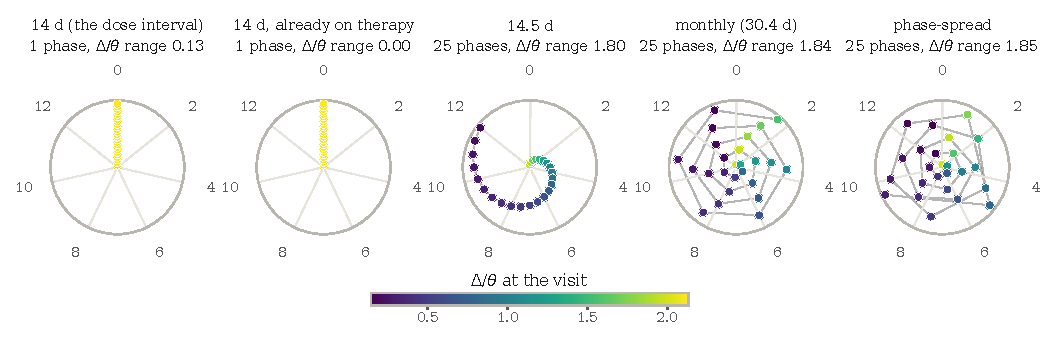
\includegraphics[width=\linewidth]{phaseclock_0920}\\[-1pt]
{\footnotesize (a) 20 Sept: polar dial, one spoke at the dose interval}
\end{minipage}\hfill
\begin{minipage}[b]{0.465\textwidth}\centering
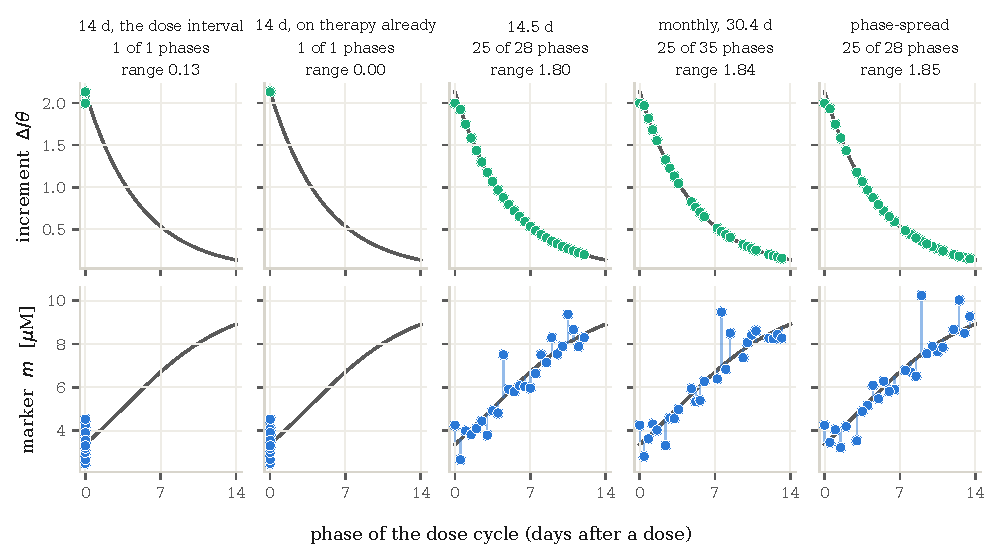
\includegraphics[width=\linewidth]{phaseclock_0927}\\[-1pt]
{\footnotesize (b) 27 Sept: increment and marker folded onto the cycle}
\end{minipage}
\caption{Figure 6 of the paper (§4.3) as it stood in each draft. Both drafts load the same
file, \texttt{results/figures/fig\_E1\_phaseclock.pdf}. That file was overwritten
\rn{git.fig6_commits} times after 20 Sept, first in \texttt{\rn{git.fig6_first}}
(\rn{git.fig6_first_date}). Each panel here is therefore regenerated by its own draft's
\texttt{audit/g1\_phase\_clock.py}, run in a temporary worktree by \texttt{fig\_phaseclock.py}.
Panel (b) shows why a phase count is not coverage. The $\rn{lnew.step_off_v}$~d schedule
reaches $\rn{new.reached_off}$ of $\rn{new.available_off}$ phases, yet over these draws it
spans only $\rn{new.range_off}$ of $\Delta/\theta$, against $\rn{new.delta_range_off}$ once
its lap is complete.}
\label{fig:clock}
\end{figure}

\W
\begin{center}\small
\begin{tabularx}{\textwidth}{@{}p{2.7cm}LL@{}}
\toprule
 & \textbf{20 Sept} & \textbf{27 Sept} \\
\midrule
Remark 4, §4.1 & ``\rn{lold.remark4_title}''; aliasing cost $\rn{old.alias_cost}\times$
 & ``\rn{lnew.remark4_title}''; lap inequality, partial-lap table, the
 $\rn{new.near_step}$~d counterexample, the $\rn{lnew.n20_n}$-visit result; aliasing cost
 unchanged at $\rn{new.alias_cost}\times$ \\
Figure 6, §4.3 & polar dial, radius $=$ visit order, one spoke at $\rn{calc.T}$~d
 & two rows (increment, marker), with headers giving phases reached of phases available \\
Tier 3, §6.4 & ``one hard exclusion'': do not sample on dosing days & ``one hard
 requirement'': complete one lap; the gap in ``avoid multiples'' is stated \\
generated numbers & no lattice or phase-clock keys & \texttt{lattice.tex} and
 \texttt{phaseclock.tex}, both new \\
\bottomrule
\end{tabularx}
\end{center}

\Out{The protocol rule is ``complete one lap of the dose cycle''. ``Avoid multiples of the
dose interval'' is necessary but not sufficient.}

% ---------------------------------------------------------------------
\section{Readouts (``sensors''): scoring table, and fusion}

\Q Which observables to use, request or exclude, and does combining them open the disease
range?

\D \emph{Sensor} and \emph{score} occur in neither draft, and \emph{fusion} only inside
\emph{infusion}. \emph{Readout} occurs in both, always for the model's observation map and
never for an observable to be scored. The readouts are scored only in
\texttt{audit/PHASE10\_SENSORS.md} (\rn{git.phase10_added}) and
\texttt{audit/q15\_sensors.py} (\rn{git.q15_added}).

\F \textbf{What the paper says}, identical in both drafts but for ``Where it changed''.
\vspace{-0.55em}
\begin{wide}
\begin{xltabular}{\linewidth}{@{}p{1.85cm}p{1.5cm}Lp{1.25cm}p{1.85cm}L@{}}
\toprule
readout & measures & literature evidence & verdict & role & key number \\
\midrule
plasma 3-HP & $m$ itself & rate ratio $\rn{lnew.rr_3hp}$ ($\rn{lnew.rr_3hp_ci_lo}$ to
 $\rn{lnew.rr_3hp_ci_hi}$) per $\rn{lnew.rr_per}\%$ lower; not a carnitine conjugate & used
 & the marker (Remark 2) & \\
C3 & propionyl\-carnitine & rate ratio $\rn{lnew.rr_c3}$, $p=\rn{lnew.p_c3}$ & excluded & none
 & co-treatment raises C3 as organic acids fall (§S1.16.2) \\
2-MC & 2-methyl\-citrate & rate ratio $\rn{lnew.rr_2mc}$, $p=\rn{lnew.p_2mc}$; tracks ammonia
 in events & excluded & none & no endpoint association \\
$1$-$^{13}$C-propionate breath & increment $\Delta$ & between-visit CV
 $\rn{lnew.breath_mean}\pm\rn{lnew.breath_sd}\%$ (range $\rn{lnew.breath_lo}$ to
 $\rn{lnew.breath_hi}\%$), \rn{lnew.breath_n} \emph{mut} MMA patients & requested
 & Tier 2, §\rn{new.sec.tier2} & needs $\le\rn{new.kappa_monthly_pct}\%$; floor crosses at
 $\rn{new.cv_floor_pct}\%$ (Table \rn{new.tab.incfloor}) \\
post-dose draw & which structure & none published & requested & Tier 1, §\rn{new.sec.tier1}
 & $\rn{new.struct_sigma_3min}\sigma$ at \rn{lnew.t_struct_t3} min,
 $\rn{new.struct_sigma_15min}$ at \rn{lnew.t_struct_t15}, $\rn{new.struct_sigma_1h}$ at
 \rn{lnew.t_struct1h} \\
IV $^{13}$C$_3$-3-HP bolus & $k_e$ & none in PA; tracer catalogued & requested & second
 anchor, Table \rn{new.tab.keprior} & to $\rn{lnew.ke_tight}\%$: $\rn{lnew.ke_gain_nom}\times$
 nominal, $\rn{lnew.ke_gain_dis}\times$ at $\rn{calc.dis_pct}\%$; exact $k_e$ leaves
 $\rn{lnew.ke_exact_left}$ \\
isotope-dilution turnover & $L+b$ & measurable in principle & closed & route 6, §\rn{new.sec.scopeprec}
 & \rn{lnew.turnover_n} visits match \rn{lnew.turnover_vs}; opens nothing below nominal \\
as-eaten diet record & $L$ & none & used & closes the fibre, Table \rn{new.tab.loadprec}
 & per-visit error $\lesssim\rn{lnew.diet_gate}\%$; at $\rn{lnew.bias_row}\%$ error,
 $\rn{new.bias_scatter_share}\%$ scatter, $\rn{new.bias_offset_share}\%$ offset \\
\bottomrule
\end{xltabular}
\end{wide}
\vspace{-0.85em}
{\small \textbf{Table A.} The paper's readouts. Sources: Remark 2, Table \rn{new.tab.require}
(§\rn{new.sec.spec}), §§\rn{new.sec.tier1} to \rn{new.sec.tier2}, §\rn{new.sec.scopeprec},
supplement §S1.14 and §S1.16.2.}

\vspace{2pt}
\noindent\textbf{What the repository has that the paper does not} (\unpub,
\rn{git.phase10_added}).
\vspace{-0.55em}
\begin{wide}
\begin{xltabular}{\linewidth}{@{}p{1.85cm}p{1.5cm}Lp{1.25cm}p{1.85cm}L@{}}
\toprule
readout & measures & literature evidence & verdict & role & key number \\
\midrule
breath test, 2-MC, C3, C3/C2, propionyl\-glycine & propionyl-CoA pool & as Table A & not
 expressible & none & \rn{audit.p10_screen_drop} of \rn{audit.p10_screen_total} candidates
 dropped: no propionyl-CoA state \\
ex vivo PCC activity (c2) & $\theta$ directly & in vivo mapping never measured in humans;
 log-sd about $\rn{audit.p10_width_w}$ & weak partner & anchor on $\theta$
 & $\rn{audit.p10_share_nom}\%$ of joint precision at nominal, $\rn{audit.p10_share_cap20}\%$
 at $\rn{audit.p10_share_capv}\%$; pair still $\rn{audit.p10_pair_lo}$ to
 $\rn{audit.p10_pair_hi}$ in the disease range; collapse mode gone,
 \rn{audit.p10_collapse_c2} against $\rn{audit.p10_collapse_lo}$ to
 $\rn{audit.p10_collapse_hi}$ of $\rn{audit.p10_collapse_n}$ \\
IV bolus (c8) & $k_e$ & as Table A & schedule first & anchor on $k_e$ & the monthly record
 misses the gate even with exact $k_e$: $\rn{audit.p10_ke_exact5}$ at $\rn{calc.dis_pct}\%$,
 $\rn{audit.p10_ke_exact10}$ at $\rn{fus.cap10}\%$ \\
turnover (c9) & $L+b$ & as Table A & dropped on size & none & an exact load buys $\rn{audit.p10_c9_lo}$ to
 $\rn{audit.p10_c9_hi}\%$; at $\rn{calc.dis_pct}\%$, $\rn{audit.p10_c9_5pct_frm}$ to
 $\rn{audit.p10_c9_5pct_to}$. Its recheck of route 6 is in \S6.2 \\
timed urine (c10) & $f_{\mathrm{renal}}k_e$ & no renal fraction for 3-HP & dominated
 & a bound only & needs $f_{\mathrm{renal}}$ to about $\rn{audit.p10_frenal}\%$ \\
\bottomrule
\end{xltabular}
\end{wide}
\vspace{-0.85em}
{\small \textbf{Table B.} \unpub: \texttt{PHASE10\_SENSORS.md} step 1, §§S.1 to S.6. In
neither draft.}

\vspace{2pt}
\noindent\textbf{Combination, the nearest thing to fusion} (\unpub).
\texttt{q15\_sensors.py} adds each sensor's precision to one diagonal of the record's Fisher
block. Rerun on the record's seeds ($\rn{fus.seed_lo}$ to $\rn{fus.seed_hi}$); c2 log-sd
$\rn{fus.p2_frac}$, c8 $\rn{fus.p8}\%$, c9 $\rn{fus.p9}\%$; entries sd$(\ln\hat\theta)$
against the $\rn{calc.gate}$ gate.
\vspace{-0.55em}
\begin{center}\small
\begin{tabular}{lcccccccc}
\toprule
capacity & record & c2 & c8 & c9 & c2+c8 & c2+c9 & c8+c9 & all \\
\midrule
$\rn{fus.cap5}\%$ & \rn{fus.rec_5} & \rn{fus.c2_5} & \rn{fus.c8_5} & \rn{fus.c9_5} & \textbf{\rn{fus.c2c8_5}}
 & \rn{fus.c2c9_5} & \rn{fus.c8c9_5} & \rn{fus.all_5} \\
$\rn{fus.cap10}\%$ & \rn{fus.rec_10} & \rn{fus.c2_10} & \rn{fus.c8_10} & \rn{fus.c9_10} & \textbf{\rn{fus.c2c8_10}}
 & \rn{fus.c2c9_10} & \rn{fus.c8c9_10} & \rn{fus.all_10} \\
\bottomrule
\end{tabular}
\end{center}
\vspace{-0.85em}
{\small \textbf{Table C.} Sensor combinations, monthly record. The rerun uses
\rn{fus.n_monthly} monthly draws, because \texttt{q15} drops the draw at $t=0$, against the
paper's \rn{calc.n_monthly}; the two are therefore not directly comparable to Table
\rn{new.tab.designs}.}

\vspace{2pt}
\noindent Only c2+c8 is worth buying, by $\rn{audit.p10_c2c8_lo}$ to
$\rn{audit.p10_c2c8_hi}\%$ over c2 alone; c9 adds nothing. Table C ranks correctly but
overstates every entry containing c2: supported width about $\rn{audit.p10_width_w}$, not
$\rn{fus.p2_frac}$. The scatter's between-patient
spread decides the rest, measurable in \rn{audit.p10_repeat_pts} patients at
\rn{audit.p10_repeat_draws} draws each. \textbf{The paper has no fusion step:} Tier 1 fixes
the structure Tiers 2 and 3 calibrate, and Tier 3 holds only if Tier 2's increment does.
\rn{lnew.six_routes} routes in §\rn{new.sec.scopeprec} are each tested and closed.

\W \textbf{Unchanged}: Remark 2, the §S1.14 marker table and the readout passages of §S1.16.2
read the same in both drafts; the C3 correction predates this window (§6.1). \emph{Tier 1:} the
27 Sept draft opens §\rn{new.sec.spec} with ``What to run first, and it is one blood draw''
(main \rn{git.main_tier1first}), and §\rn{new.sec.tier1} now calls Tier 1 a \emph{structure}
test, not a fit threshold.
\emph{Tier 2, §\rn{new.sec.tier2}:} the Table \rn{new.tab.incfloor} floors and the
$\rn{new.tier1_visits_at_pub}$-draw count are now generated (\texttt{\rn{gen.tier1}}), values
unchanged; Table \rn{new.tab.keprior} unchanged. \emph{§\rn{new.sec.scopeprec}:} the diet
values moved (§6); route 6 keeps the below-nominal clause Table B could not reproduce.

\Out{Three readouts are used or requested, gated in sequence. The combination analysis exists
only in the audit, and the combinations that reach the gate in Table C do so only at an assay
width nobody can currently deliver: at the supported width the best pair still runs
$\rn{audit.p10_pair_lo}$ to $\rn{audit.p10_pair_hi}$ across the disease range.}

% ---------------------------------------------------------------------
\section{Was a genetic prior helpful?}

\Q Can genotype supply what the marker record cannot, either as a prior on $\theta$ itself
or as an anchor for $k_e$?

\D Read §S1.10, Proposition 6 (§S1.18.1), Remark 14 (§S1.16.3), Remarks 21 and 22
(§S1.16.7) and Table 11 (§6.3). Recomputed the anchor's crossing from the model constants.
Searched the repository for a genotype-informed prior on $\theta$.

\F \textbf{What the paper says.} Three findings, all identical in both drafts.
\begin{itemize}
\item \textbf{The founder population is ideal for the map and closed to the design}
(§S1.10). \emph{PCCA} c.425G$>$A accounts for $\rn{lnew.saudi_founder}\%$ of families, with
one compound-heterozygous family, so genotype to capacity is unconfounded. The series is
$\rn{lnew.saudi_pcca}\%$ \emph{PCCA} (\rn{lnew.saudi_pcca_n} patients), and §6.5 requires a
therapeutic increment that varies, which no patient outside the trial receives. The two
criteria select different cohorts, and the paper leaves the genotype argument as a property
of the literature rather than a recommendation.
\item \textbf{The null-genotype anchor inverts with severity} (Remarks 21 and 22). A patient
with $\theta = 0$ gives $s = k_e m$, which fixes $k_e$ and collapses the fibre to a point. Its
amplification of a load error crosses one at $\theta = 2k_e(K_m+\bar m)$, which the model
constants put at $\rn{calc.null_cross}$ (the paper writes $\approx\rn{lnew.null_cross}$), and
reaches $\rn{calc.null_amp300}$ at the parent model's $\theta = \rn{lnew.theta_parent}$ (paper:
$\rn{lnew.null_amp}$). The anchor attenuates the error for mild patients and amplifies it for
severe ones.
\item \textbf{Knowing $k_e$, which is what such an anchor supplies, does not close the gate}
(Table 11). Tightening from the published prior to $\rn{lnew.ke_tight}\%$ is worth
$\rn{lnew.ke_gain_nom}\times$ at nominal capacity and $\rn{lnew.ke_gain_dis}\times$ at
$\rn{calc.dis_pct}\%$ of it, but an exact $k_e$ still leaves $\rn{lnew.ke_exact_left}$ against
the $\rn{calc.gate}$ gate.
\end{itemize}
\noindent A genotype-informed prior on $\theta$ itself: \nf, in either draft.

\medskip
\noindent\textbf{What the repository has that the paper does not} (\unpub).
\begin{center}\footnotesize
\begin{tabularx}{\textwidth}{@{}p{3.0cm}LL@{}}
\toprule
item & what it establishes & the limit it states \\
\midrule
ex vivo assay as a prior on $\theta$, \texttt{q5\_exvivo\_prior.py} (\rn{git.q5_added})
 & An assay on the patient's own cells is carried as a log-normal prior of width
 $\rn{audit.r58_width_lo}$ to $\rn{audit.r58_width_hi}$. It adds to the record in exact
 quadrature, proven from the Schur complement and confirmed in all $\rn{audit.r58_cells}$
 cells, so assay and record cannot spoil each other. With $k_e$ measured it changes
 \rn{audit.r58_verdicts_n} verdicts, all at a prior of $\rn{audit.r58_verdicts_w}$, the
 practical one turning monthly sampling at $\rn{fus.cap10}\%$ of normal from
 $\rn{audit.r58_10pct_frm}$ into $\rn{audit.r58_10pct_to}$.
 & Without a $k_e$ measurement the combined figure sits at $\rn{audit.r58_dom_comb}$ against
 the assay's own $\rn{audit.r58_dom_width}$ at $\rn{calc.dis_pct}\%$, so the record adds under
 one per cent and the answer is the assay's. The risk sits where the benefit does: at
 $\rn{calc.dis_pct}\%$, $\rn{audit.r58_centring_lo}$ to $\rn{audit.r58_centring_hi}\%$ of a
 centring error passes into $\hat\theta$; at $\rn{fus.cap10}\%$ a prior wrong by a factor of
 two is worth nothing, RMSE $\rn{audit.r58_rmse_w}$ with it against
 $\rn{audit.r58_rmse_wo}$ without. \\
\addlinespace
review of an external genotype-prior document, \texttt{PHASE12\_GENOTYPE\_REVIEW.md}
 (\rn{git.phase12_added})
 & The document's breath-test figure, $\rn{audit.p12_imported_ctrl}\%$ controls and
 $\rn{audit.p12_imported_pat}\%$ patients, is the retracted one and is not imported. The
 repository's own $\rn{audit.p12_kappa}$, which sizes Tier 2 and with it the
 $\rn{audit.p12_draws}$-draw count, is graded
 \textsc{\rn{audit.p12_status_label}}: two independent secondary readings agree and no primary
 read has been made here.
 & Nothing from the document enters the repository, and the grading is a status label rather
 than a new number. It changes no value in either draft. \\
\bottomrule
\end{tabularx}
\end{center}
\vspace{-0.4em}
{\small \textbf{Table D.} Genotype-adjacent analysis in the repository at 27 Sept, in neither
draft. Sources: \texttt{REVIEW\_LOG.md} R58 and \texttt{audit/PHASE12\_GENOTYPE\_REVIEW.md}.}

\W Nowhere in the paper. §S1.10, Remarks 21 and 22 and Table 11 are unchanged between the
drafts. The only edit anywhere near this material is a pointer in §6.6, where ``supplement,
\S S1'' became ``\S S1.16.7''.

\Out{A genetic prior helps most where it is needed least: the anchor attenuates a load error
for the mild patient and amplifies it for the severe one.}

% ---------------------------------------------------------------------
\section{Delivery and administration: the analysis was there, the conclusion is new}

\Q Should the dosing schedule, and not only the sampling schedule, be designed for
identification?

\D Every case was priced on 20 Sept and stands unchanged on 27 Sept: amplitude alternation,
a longer and a shorter interval, continuous delivery at the same rate, a $D$ sweep from
$\rn{lnew.dsweep_range_lo}$ to $\rn{lnew.dsweep_range_hi}$, and \rn{lnew.dosesens_n}
readings of the dose calibration in Table~\rn{new.tab.dosesens}. New this week: the exposure sweep to the continuous limit
(\texttt{\rn{gen.therapy}}, on main \rn{git.main_exposure}) and the three named readings of
the admissibility bound (\rn{git.main_readings}).

\F Every case above the rule stands in both drafts at the same value. The rows below it
are new.
\vspace{-2pt}
\begin{wide}
\begin{tabularx}{\linewidth}{@{}p{3.0cm}Lp{2.45cm}@{}}
\toprule
case & result & status \\
\midrule
$\pm\rn{lnew.alt_amp}\%$ amplitude alternation & $\rn{lnew.alt_gain}\%$ of precision for a
 $\rn{lnew.alt_cut}\%$ cut in the trough & carried, \S\rn{new.sec.route} \\
a \rn{lnew.h28_word}-day interval & $\rn{lnew.h28_gain}\%$ for an $\rn{lnew.h28_cut}\%$ cut
 & carried, \S\rn{new.sec.route} \\
a \rn{lnew.h7_word}-day interval & doubles the trough, costs $\rn{lnew.h7_cost}\%$
 & carried, \S\rn{new.sec.route} \\
continuous infusion & no trough, no excitation: the identification stops existing
 & carried, \S\rn{new.sec.route} \\
booked $D = \rn{calc.D}$ at nominal capacity & $\rn{new.sd_monthly}$ against a sweep best of
 $\rn{lnew.dsweep_nom_best}$: within \rn{lnew.dsweep_within} per cent of optimal
 & carried, \S\rn{new.sec.scopeprec} \\
best $D$ in the disease range & $\rn{lnew.dsweep_dis_best}$ at
 $D\approx\rn{lnew.dsweep_dis_d}$ against $\rn{lnew.dsweep_dis_booked}$ booked: no dose
 opens a window & carried, \S\rn{new.sec.scopeprec} \\
largest admissible $D$ at $\rn{calc.dis_pct}\%$ & $\rn{lnew.dmax_5pct}$, where the booked
 increment drives the enzyme to $\rn{lnew.enzyme_x_normal}$ times normal; the monthly design
 still returns $\rn{lnew.d2672_sd}$ & value carried, reading new \\
\midrule
\textbf{no interior optimum} & marker exposure falls monotonically to the continuous limit,
 $\Delta\to\rn{new.delta_cont}$: by $\rn{new.exp_fall_nominal}\times$ at nominal
 ($\rn{new.exp_h28_nominal}$ to $\rn{new.exp_cont_nominal}$) and
 $\rn{new.exp_fall_disease}\times$ at $\rn{calc.dis_pct}\%$ ($\rn{new.exp_h28_disease}$ to
 $\rn{new.exp_cont_disease}$). Peak marker and admissibility ratio fall with it
 & \textbf{new}, \S\rn{new.sec.route} \\
\textbf{three readings of the bound} & R1 (inferred normal, dose scaled with $\theta$):
 constant $\rn{new.adm_r1}$, blind to a breach below $\rn{new.ceiling_blind_pct}\%$
 residual. R2 (inferred normal, booked dose): $\rn{new.adm_r2_20}$ rising to
 $\rn{new.adm_r2_10}$ as capacity halves, the one reading that crosses the bound. R3
 (normal fixed at $\rn{calc.theta}$): breaches at every capacity, $\rn{new.adm_r3_100}$ at
 normal. The readings coincide only at $\theta=\rn{calc.theta}$ and
 $\theta=\rn{calc.theta_dis}$; both anchor numbers sit on the latter. The paper reports on
 R2 & \textbf{new}, \S\rn{new.sec.scopeprec} \\
\bottomrule
\end{tabularx}
\end{wide}

\W \emph{\S\rn{new.sec.route}:} new text inside the administration-route paragraph, on the
absence of an interior optimum; the rest, the delivery cases included, is the 20 Sept text. \emph{\S\rn{new.sec.scopeprec}:}
the bound gained the R1/R2/R3 table and the paragraph naming where the readings coincide; the
$D$ sweep and its two values carry over. \emph{Table \rn{new.tab.dosesens}}
(\S\rn{new.sec.admiss}, the dose calibration) is unchanged.

\Out{Optimise the sampling schedule, which is free. Leave the dosing schedule to therapeutic
judgment, and check identifiability before any move to continuous delivery.}

% ---------------------------------------------------------------------
\section{$A$, $B$, $C$ and what they mean (new figures)}

\Q What does each invariant mean, and why is the capacity the one that disappears?

\D Both figures come from \texttt{fig\_abc.py} and the repository's model code at the
Table~\rn{new.tab.params} constants $\theta=\rn{calc.theta}$, $K_m=\rn{calc.Km}$,
$k_e=\rn{calc.ke}$, $\bar m=\rn{calc.mbar}$, $D=\rn{calc.D}$, $T=\rn{calc.T}$~d,
$t_{1/2}=\rn{calc.thalf}$~d, $L=\theta g(\bar m)+k_e\bar m=\rn{calc.L}$. The balance
$L+b=(\theta+\Delta)m/(K_m+m)+k_e m$ gives $\Delta(m)=A/m+B+Cm$, $A=K_m(L+b)$,
$B=L+b-\theta-k_eK_m$, $C=-k_e$.

\F Every check value reproduces: $A=\rn{calc.A}$, $B=\rn{calc.B}$, $C=\rn{calc.C}$, untreated
$m=\rn{calc.m_untreated}$, $\Delta(\rn{calc.mwf})=\rn{calc.delta6}$.\footnote{The check value
supplied for $\Delta(\rn{calc.mwf})$ disagrees with the repository; the repository's value is
printed, and the closing list records it.} At $\theta=\rn{calc.theta_dis}$:
$B=\rn{calc.B_dis}$, untreated $m=\rn{calc.m_untreated_dis}$, a ratio of
$\rn{calc.m_ratio_dis}$, matching the $\rn{lnew.scope_5pct_ratio}\times$ of
Table~\rn{new.tab.scope}. The twin at $b=\rn{calc.twin_b_last}$: $\theta=\rn{calc.twin400_theta}$,
$K_m=\rn{calc.twin400_km}$, relaxation $\rn{calc.relax_b400}$ against
$\rn{calc.relax_b0}$~d$^{-1}$, the paper's own two values in \S\rn{new.sec.collapse}
($\rn{lnew.relax_b400}$, $\rn{lnew.relax_b0}$).

\begingroup\footnotesize\centering
\begin{minipage}[t]{0.38\textwidth}\vspace{0pt}
\centering
\begin{tabular}{@{}lcccl@{}}
\toprule
parameter & $A$ & $B$ & $C$ & reading \\
\midrule
$\theta$ & & $\bullet$ & & own enzyme \\
$K_m$ & $\bullet$ & $\bullet$ & & half-saturation \\
$k_e$ & & $\bullet$ & $\bullet$ & backup route \\
$b$ & $\bullet$ & $\bullet$ & & diary error \\
\bottomrule
\end{tabular}
\end{minipage}\hfill
\begin{minipage}[t]{0.59\textwidth}\vspace{0pt}
\begin{tabularx}{\textwidth}{@{}lL@{}}
\toprule
invariant & what it is, and its size \\
\midrule
$A=K_m(L+b)$ & load $\times$ half-saturation: $+\rn{calc.A_over_6}$ at
$m=\rn{calc.mwf}$, the largest term \\
$B=L+b-\theta-k_eK_m$ & the only place $\theta$ appears: at $\theta=\rn{calc.theta_dis}$ the
smallest of $+\rn{calc.Bp_load}$, $-\rn{calc.theta_dis}$, $-\rn{calc.keKm}$, the scope limit of
\S\rn{new.sec.scopeprec} \\
$C=-k_e$ & the backup route: bend $\rn{calc.bend}$ over $m=\rn{calc.m_lo}$ to
$\rn{calc.m_hi}$ against $\rn{calc.diary_move}$ per $\rn{calc.unit_b}\,\mu$M/d of diary error,
so $k_e$ comes from a prior \\
\bottomrule
\end{tabularx}
\end{minipage}\par\endgroup

\begin{figure}[htbp]
\centering
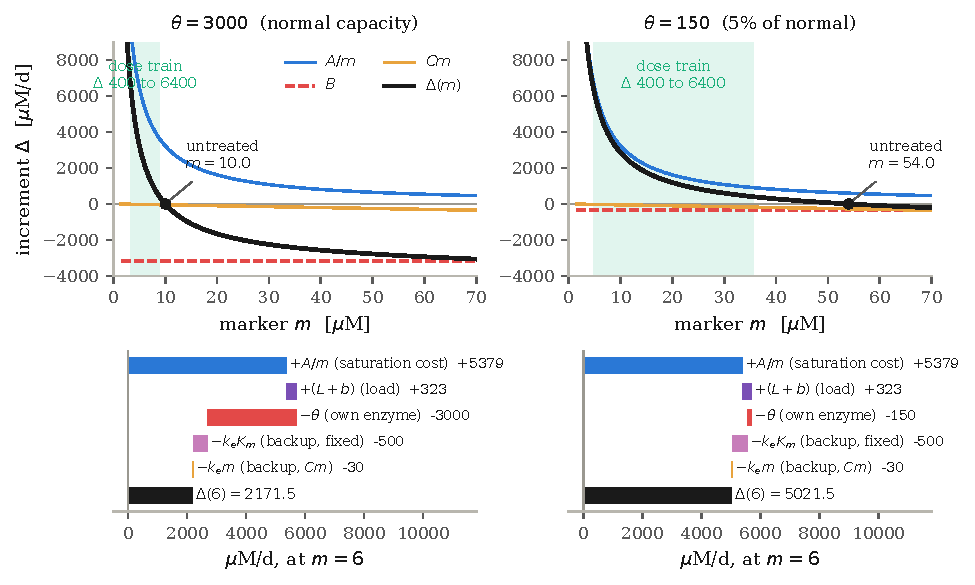
\includegraphics[width=0.80\textwidth]{fig5a_abc}
\caption{$\Delta(m)$ decomposed at $\theta=\rn{calc.theta}$ (left) and $\rn{calc.theta_dis}$
(right). Green: the dose train's range, $\Delta$ from $\rn{calc.trough}$ to $\rn{calc.peak}$.
Below, a waterfall at $m=\rn{calc.mwf}$: $A$ blue, $B$'s pieces purple, red, pink, $C$ amber.
$-\theta$ is $B$'s largest piece at normal capacity, its smallest at $\rn{calc.dis_pct}\%$.}
\label{fig:abc}
\end{figure}

\begin{figure}[htbp]
\centering
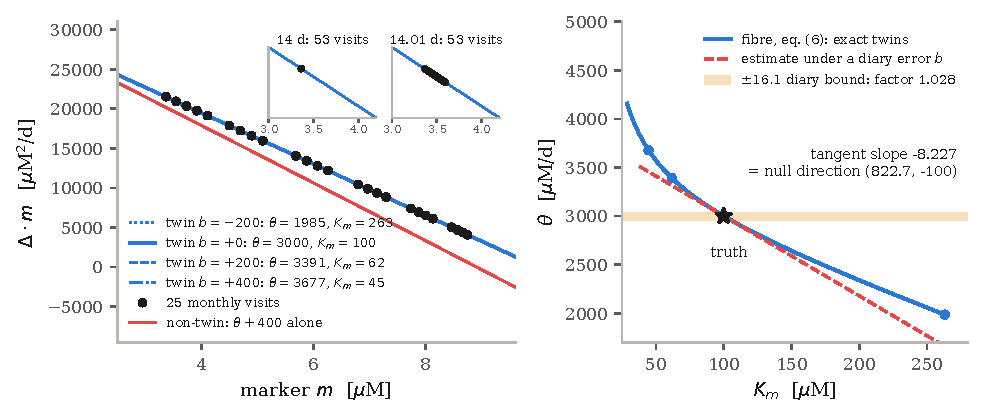
\includegraphics[width=0.80\textwidth]{fig5b_fibre}
\caption{Left: the record as a parabola, $\Delta m = A+Bm+Cm^2$. The \rn{calc.n_monthly}
monthly visits and the twins at $b\in\{\rn{calc.twin_bs}\}$ draw one curve; moving $\theta$
alone by $\rn{calc.nontwin_dtheta}$ does not. Insets: the aliased designs, one point every
$\rn{calc.T}$~d, a cluster every $\rn{new.near_step}$~d. Right: the fibre is curved, but
estimates under a constant diary error, $\hat K_m=K_m(1+b/L)$,
$\hat\theta=\theta-b(1+K_mk_e/L)$, lie on a line of slope $\rn{calc.locus_slope}$, tangent at
the truth along the rank proposition's null vector
$(\rn{calc.null_theta},\rn{calc.null_km})$. Shaded: the $\pm\rn{calc.diary_b}$ bound from the
$\rn{calc.load_pct}\%$ diary record, a factor of $\rn{calc.diary_factor}$ on $\theta$.}
\label{fig:fibre}
\end{figure}

\W Nothing: the increment law, the fibre and the invariants read the same in both drafts. The
27 Sept \S\rn{new.sec.destroys} adds the affine map $\hat\theta=\theta-\rn{new.bias_slope}\,b$
and the Vandermonde reading of the invariants. \textbf{The tangent reading is in neither
draft:} Figure~\ref{fig:fibre} puts estimates under a constant diary error on the fibre's
tangent at the truth, the rank proposition's null direction. One sentence for
\S\rn{new.sec.destroys}:
\begin{quote}\small
``The fibre is curved in $(K_m,\theta)$, but a constant load bias moves the estimate along its
tangent at the truth, Proposition~\textbackslash ref\{prop:rank\}'s null direction, so a bound
on $b$ leaves a segment of that tangent and the factor on $\theta$ is exact, not linearised.''
\end{quote}

\Out{$\theta$ lives in one invariant, beside two larger terms in the disease range: the scope
limit in a line of algebra.}

% ---------------------------------------------------------------------
\section{Other changes with a concrete outcome}

\Q Which other claims changed status in this window, and what replaced each one?

\D Listed every \emph{As corrected} and \emph{withdrawn} passage in both main texts and in
supplement §§S1.15, S1.16.2 and S1.20, and every new result, from \texttt{git diff} between
the two commits. Each row is dated twice: when the passage was first written, and when it
reached main.

\subsection{Corrections ledger, 20 to 28 September}
\begin{center}\footnotesize
\begin{tabularx}{\textwidth}{@{}p{2.6cm}LLp{3.1cm}@{}}
\toprule
change & 20 Sept & 27 Sept & outcome \\
\midrule
carnitine timescale, §2.3 and §S1.15 (main \rn{git.main_carn})
 & ``\rn{lnew.carn_old_claim}'' & withdrawn: the reduction needs the other separation, and
 $\tau_c/\tau_m$ spans $\rn{lnew.tauc_ratio_lo}$ to $\rn{lnew.tauc_ratio_hi}$ over the sampled
 region, so carnitine is the slower state & the reduction stands as an identity at
 equilibrium, not as a timescale argument \\
``the reduction is verified'', §2.3 and §2.6 (main \rn{git.main_verified})
 & ``\rn{lnew.verified_old_claim}'' & withdrawn: the agreement is the identity
 $\dot c = 0$ at a fixed point, so it cannot fail at any parameter value & the three tests are
 kept as regression tests on the arithmetic, and none is evidence for the premise \\
separatrix as a lower bound, §2.3 (main \rn{git.main_separatrix})
 & a lower bound on the true basin, as recorded in \rn{lnew.r22} of the review log
 & withdrawn: it bounds from above the manifold only. From a pool depleted to
 $\rn{lnew.sep_depleted_fill}$, $0.5$ and $0.25$ of $c^{\ast}(m)$ the boundary falls
 $\rn{lnew.sep_depleted_a}\%$, $\rn{lnew.sep_depleted_b}\%$ and $\rn{lnew.sep_depleted_c}\%$
 \emph{below} it & the basin boundary is a curve in $(m,c)$, and the reduced separatrix is one
 point on it, not a bound either way \\
two tests and the closed form, §2.6 (main \rn{git.main_numerics})
 & the closed form's validity is ``measured rather than assumed'' & withdrawn: neither test
 touches the two-state system & what the premise costs is bounded in the $k$ row of §S2
 instead \\
factor of $\rn{lnew.factor24_old}$ on $\theta_{\mathrm{crit}}$, §1 and §S1.20
 (main \rn{git.main_factor24}) & stood in the introduction and in §S1.20; count in §1:
 \rn{lold.factor24_count} & withdrawn: it had no derivation, and none of the
 $\rn{lnew.pairs_181}$ pairs of stated endpoints reproduces it; count in §1:
 \rn{lnew.factor24_count} & replaced by the margin window, $\rn{new.mtol_window_lo_pct}\%$ of
 its centre at $m_{\mathrm{tol}}=\rn{lnew.mtol_a}$, $\rn{new.mtol_window_pct}\%$ at
 $\rn{lnew.mtol_b}$ and $\rn{new.mtol_window_hi_pct}\%$ at $\rn{lnew.mtol_c}$, which a
 clinician can compute per patient \\
crisis-regime threshold, §5 (main \rn{git.main_crisis})
 & a regret-equalised boundary at $\rn{lold.crisis_threshold}\,\theta$; count in §5:
 \rn{lold.crisis039_count} & withdrawn: once the fit collapses, $\hat\mu$ reports how far
 $\hat K_m$ has departed, by factors from about \rn{lnew.crisis_km_lo} upwards, rather than the
 decision; count: \rn{lnew.crisis039_count} & no threshold is quoted for the crisis regimes,
 because there is nothing there for one to find \\
decision error rates, §5 & $\rho=1$ errs at $\rn{lold.dec_rho1_err}\%$, median
 $\hat\theta/\theta$ of $\rn{lold.dec_rho1_med}$ & recomputed over \rn{lnew.seeds_n} seeds at
 \rn{lnew.seeds_reps} replicates each: $\rn{lnew.dec_rho1_err}\%$, median
 $\rn{lnew.dec_rho1_med}$, each with its range & the seed spread is now reported, and the
 partial-recording cell is named as the least stable of the four \\
\bottomrule
\end{tabularx}
\end{center}

\subsection{Recent corrections outside the window}
Two corrections the request placed in this window are older, and both are already in the
20 Sept draft, word for word.
\begin{itemize}
\item \textbf{C3's exclusion rests on the co-treatment ground alone} (§S1.16.2). Entered
\rn{git.c3_date} in \texttt{\rn{git.c3_commit}}, a day before the 20 Sept snapshot.
\item \textbf{The assay term dominates the load term in $\sigma$} wherever the load is
recorded better than about the assay's own CV, $\rn{lnew.assay_vs_load_assay}$ against
$\rn{lnew.assay_vs_load_load}$ at a $2\%$ load record (§S1.16.7). Recorded in the review log
on \rn{git.assay_date} in \texttt{\rn{git.assay_commit}}.
\end{itemize}

\subsection{New results}
\begin{center}\footnotesize
\begin{tabularx}{\textwidth}{@{}p{2.6cm}LLp{3.1cm}@{}}
\toprule
result & 20 Sept & 27 Sept & outcome \\
\midrule
affine load-bias map, §3.1 & the factor $\rn{lold.bias_theta_factor}$ is quoted
 & $\hat\theta=\theta-\rn{new.bias_slope}\,b$ exactly, at every $b$ and with no higher-order
 term & what a bound on $b$ leaves open in $\theta$ is arithmetic, not a linearisation:
 $\rn{new.bias_theta_factor}$ \\
admissibility readings, §7.1 (main \rn{git.main_readings})
 & one bound, its reading implicit & R1, R2, R3 named and tabulated, with the two points where
 they coincide & every verdict now names its reading, and the paper reports on R2 \\
the §8.1 boundary fit (main \rn{git.main_boundary})
 & $\hat\theta=\rn{lold.fit_theta_hat}$ against a true $\rn{lnew.theta_parent}$; margin
 $+\rn{lold.fit_margin_true}$ to $+\rn{lold.fit_margin_est}$
 & $\rn{new.fit_theta_hat}$ is a \emph{boundary} solution, with $\hat k_e$ on its bound at
 $\rn{new.fit_ke_hat}$; released it goes to $\rn{new.fit_ke_hat_free}$ and $\hat\theta$ to
 $\rn{new.fit_theta_hat_free_ke}$. Across fit definitions the margin spans
 $\rn{lnew.margin_lo}$ to $+\rn{lnew.margin_hi}$ & a boundary solution is not a point estimate,
 so the gap is not a margin. The design's operating points are bounded away from the problem:
 $L/k_e=\rn{new.local_ceiling}$ against $\sqrt{K_cM_i}=\rn{new.peak_floor}$ \\
§8.3, new (main \rn{git.main_pattern2}) & --- & two misspecifications with opposite signs: one
 returns $\theta$ too high by $\rn{lnew.misspec_high_lo}$ to $\rn{lnew.misspec_high_hi}\times$,
 the other too low ($\rn{new.fit_theta_hat}$ against $\rn{lnew.theta_parent}$), and both leave a
 residual inside the noise the specification already asks for
 ($\rn{new.fit_resid_sigma}\sigma$) & residual size does not bound structural error, which is
 why Tier 1 is a structure test and not a goodness-of-fit threshold \\
decompensation route, §8.1 & excluded \rn{lold.excluded_twice} over
 & \rn{lnew.excluded_three}: the excursion is not observed at the magnitude required, the
 model does not hold there, and the reduction carries no warrant there either, the two
 formulations differing by $\rn{lnew.reduction_gap_lo}$ to $\rn{lnew.reduction_gap_hi}\%$ and
 the basin by up to $\rn{lnew.basin_max}\%$ & the route is excluded on three independent
 grounds, not narrowly missed \\
§S4, new (main \rn{git.main_s4}) & the evidence column was generated and never input
 & ``\rn{lnew.s4_title}'' & the promise Table 4's caption makes is kept \\
wired literals & diet gains printed as $\rn{lold.diet_gain15_pct}\%$ and
 $\rn{lold.diet_gain50_pct}\%$ & generated: $\rn{new.diet_gain15_pct}\%$ and
 $\rn{new.diet_gain50_pct}\%$ & two printed values moved when they were wired to their
 generator \\
\bottomrule
\end{tabularx}
\end{center}
\noindent The review log carries \rn{lnew.r22} (the separatrix), R152 (six numbers files
generated and never loaded), R155 (the retitling, and Tier 1 stated first), R158 (§S4) and
R182 (the supplement's own title).
\textbf{One gap to flag.} The margin window is in the introduction, which carries
\rn{lnew.mtolwin_in_question} of its generated keys, and not in the abstract, which carries
\rn{lnew.mtolwin_in_abstract}. The abstract therefore has no replacement for the withdrawn
factor. The window's values were already generated on 20 Sept
($\rn{old.mtol_window_pct}\%$ at $\rn{lnew.mtol_b}$) and simply not printed.

\subsection{Audit results not in the paper}
\begin{center}\footnotesize
\begin{tabularx}{\textwidth}{@{}p{2.9cm}LLp{2.6cm}@{}}
\toprule
item & what it establishes & what publishing it would change & where it would go \\
\midrule
readout screen, \texttt{PHASE10\_SENSORS.md} step 1 (\rn{git.phase10_added})
 & \rn{audit.p10_screen_drop} of \rn{audit.p10_screen_total} candidate observables cannot be
 expressed in this model at all, because it has no propionyl-CoA state
 & the paper excludes C3 and 2-MC on the endpoint and on co-treatment; this is a second and
 structural reason, and it also bounds what any future marker panel could add without a new
 state & Remark 2 (§2.5), or §S1.14 beside the table of what is known \\
sensor pricing and combinations, §§S.1 to S.4 (same file)
 & only c2+c8 is worth buying, by $\rn{audit.p10_c2c8_lo}$ to $\rn{audit.p10_c2c8_hi}\%$ over
 c2 alone; c9 is redundant in every combination; the monthly record misses the gate at
 $\rn{calc.dis_pct}\%$ even with exact $k_e$ ($\rn{audit.p10_ke_exact5}$)
 & it prices the anchors jointly, where §7.1 closes them one at a time, and it puts the
 schedule decision before the sensor decision & §7.1, as a joint row under the
 \rn{lnew.six_routes} closed routes \\
route 6 recheck (same file, §S.1b)
 & at nominal, \rn{audit.p10_r6_nom_audit} measured-load visits match the record, against the
 paper's \rn{audit.p10_r6_nom_paper}; below nominal the count is
 \rn{audit.p10_r6_below_audit} and flat, not the paper's \rn{audit.p10_r6_below_paper}
 & one supporting number in route 6 would change; the finding it supports, that the route opens
 nothing below nominal, is unaffected & §7.1, route 6 \\
ex vivo prior on $\theta$, \texttt{q5\_exvivo\_prior.py} (\rn{git.q5_added})
 & prior and record add in exact quadrature; at $\rn{calc.dis_pct}\%$ a tight prior transmits
 $\rn{audit.r58_centring_lo}$ to $\rn{audit.r58_centring_hi}\%$ of any centring error, and at
 $\rn{fus.cap10}\%$ a prior wrong by a factor of two is worth nothing
 & it would give the paper a stated position on whether a direct enzyme assay may enter the
 estimator, which neither draft takes & §6.3, beside Table 11's second anchor \\
genotype-document review, \texttt{PHASE12\_GENOTYPE\_REVIEW.md} (\rn{git.phase12_added})
 & $\rn{audit.p12_kappa}$, which sizes Tier 2 and the $\rn{audit.p12_draws}$-draw count, is
 \textsc{\rn{audit.p12_status_label}}
 & it would put a verification status on the one literature figure the specification's headline
 count rests on & §6.3, or the $\kappa$ row of the §S2 registry \\
\bottomrule
\end{tabularx}
\end{center}
\noindent These are recorded as what exists and where it would fit. Nothing here is a
recommendation to publish.

\Out{Six claims were withdrawn or corrected in the window, and each left a narrower statement
a reader can check; three analyses that bear on the paper's own sections sit in the audit
unpublished.}

% ---------------------------------------------------------------------
\section*{What this report could not trace, and what it checked and rejected}
\addcontentsline{toc}{section}{Untraced}

\noindent\textbf{Asserted here without a source in the repository.} One item.
\begin{itemize}
\item The proposed sentence for §3.1 in §5 is this report's own wording. The reading behind
it, that the estimate locus is the fibre's tangent along Proposition 4's null direction, is
computed by \texttt{fig\_abc.py} from the model code, but no passage in either draft states
it.
\end{itemize}

\noindent\textbf{Checked against the repository and rejected.} Six claims in the request did
not survive; the repository's reading is used above.
\begin{enumerate}
\item \emph{The C3 correction is new on 27 Sept.} It is not. Both drafts carry the passage
word for word, from \texttt{\rn{git.c3_commit}} on \rn{git.c3_date}.
\item \emph{The assay-versus-load correction is new on 27 Sept.} It is not. Both drafts print
$\rn{lold.assay_vs_load_assay}$ against $\rn{lold.assay_vs_load_load}$, and the review log
records it from \rn{git.assay_date}.
\item \emph{Supplement §S1.16.7 carries a correction.} It carries no \emph{As corrected} or
\emph{withdrawn} passage in either draft. Its only edit in the window is the wiring of
$\rn{new.sd_monthly}$, which the 20 Sept text printed as $\rn{lold.sd_monthly_lit}$.
\item \emph{$\Delta(6)=2171$.} The repository gives $\rn{calc.delta6}$.
\item \emph{The delivery results are new.} The $\pm\rn{lnew.alt_amp}\%$ alternation, the
\rn{lnew.h28_word}- and \rn{lnew.h7_word}-day intervals, the $D$ sweep and
$D=\rn{lnew.dmax_5pct}$ are all in the 20 Sept draft at the same values. Only the
interior-optimum paragraph and the R1/R2/R3 reading are new.
\item \emph{A separate readout scoring underlies the paper.} \emph{Sensor}, \emph{fusion},
\emph{readout} and \emph{score} appear nowhere in either draft. The scoring exists only in
\texttt{audit/PHASE10\_SENSORS.md} (\rn{git.phase10_added}), after the 20 Sept snapshot and
in neither document.
\end{enumerate}

\noindent\textbf{Searched for and not found.} A genotype-informed prior on $\theta$: \nf. The
nearest items are the ex vivo assay prior and the genotype-document review of §3, neither of
which is in either draft.

\medskip
\noindent\rule{\textwidth}{0.4pt}\\[2pt]
{\footnotesize The two states compared are \texttt{\rn{git.old}} (\rn{git.old_date}) and
\texttt{\rn{git.new}} (\rn{git.new_date}), each the last commit on or before its date. No
file under \texttt{paper/} changed after the later of these
(\rn{git.paper_untouched_after_new} files), so this report's own commits do not affect the
comparison. Numbers: \texttt{make\_numbers.py}, with \texttt{provenance.csv} giving the source
of each. Figures: \texttt{fig\_phaseclock.py} and \texttt{fig\_abc.py}. Nothing in
\texttt{paper/} was edited.}


\end{document}
